\documentclass[abstract=on,10pt,a4paper,bibliography=totocnumbered]{article}
\usepackage[paper=a4paper,left=35mm,right=35mm,top=25mm,bottom=30mm]{geometry}
\usepackage[doublespacing]{setspace}
\usepackage[english]{babel}
\usepackage[utf8]{inputenc}
\usepackage{amsmath}
\usepackage{colortbl}
\usepackage{amsfonts}
\usepackage{amssymb}
\usepackage{gensymb}
\usepackage{textcomp}
\usepackage{graphicx}
\usepackage{tikz}
\usepackage{enumerate}
\usepackage{enumitem}
\usepackage{subcaption}
\usepackage{booktabs}
\usepackage[hidelinks]{hyperref}
\usepackage[nameinlink]{cleveref}
\usepackage{multirow}
\usepackage{arydshln}
\usepackage[flushleft]{threeparttable}
% \usepackage[nomarkers, nolists]{endfloat}
\usepackage{scalerel}
\usepackage{makecell}
\usepackage{ifthen}
\usepackage{tikz}
\usepackage{lineno}
\usetikzlibrary{svg.path}

%------------------------------------------------------------------------------
%  Bibtex vs Biblatex
%------------------------------------------------------------------------------
% While bibtex is very nice to use, it's insanely slow. I therefore work with
% bibtex until the final stage. Set the value below to "true" or "false" to pick
% which one should be used.
\newboolean{usebiblatex}
\setboolean{usebiblatex}{true}

% Depending on the question, the commands below will prepare the document
% accordingly
\ifthenelse{\boolean{usebiblatex}}{
  %-----------------------------------------------------------------------------
  %  If using biblatex
  %-----------------------------------------------------------------------------
  % Load required packages and refer to correct bibliography
  \usepackage{csquotes}
  \usepackage[
      backend=biber
    , style=apa          % To display Author-year in the text
    , natbib=true        % Necessary to use citep, etc.
    , hyperref=true      % To have clickable links in the references
    , useeditor=false    % Don't add editor to publications
    , sorting=ynt        % Sort by year, name, and title
    , uniquename=false   % Avoid that initials are put
  ]{biblatex}
  \addbibresource{Literature.bib}

  % To include author in link
  \DeclareFieldFormat{citehyperref}{%
  \DeclareFieldAlias{bibhyperref}{noformat}% Avoid nested links
  \bibhyperref{#1}}
  \DeclareFieldFormat{textcitehyperref}{%
  \DeclareFieldAlias{bibhyperref}{noformat}% Avoid nested links
  \bibhyperref{%
    #1%
    \ifbool{cbx:parens}
      {\bibcloseparen\global\boolfalse{cbx:parens}}
      {}}}
  \savebibmacro{cite}
  \savebibmacro{textcite}
  \renewbibmacro*{cite}{%
    \printtext[citehyperref]{%
      \restorebibmacro{cite}%
      \usebibmacro{cite}}}
  \renewbibmacro*{textcite}{%
    \ifboolexpr{
      ( not test {\iffieldundef{prenote}} and
        test {\ifnumequal{\value{citecount}}{1}} )
      or
      ( not test {\iffieldundef{postnote}} and
        test {\ifnumequal{\value{citecount}}{\value{citetotal}}} )
    }
      {\DeclareFieldAlias{textcitehyperref}{noformat}}
      {}%
    \printtext[textcitehyperref]{%
      \restorebibmacro{textcite}%
      \usebibmacro{textcite}}}

  % Remove editor form everything but books
  \AtEveryBibitem{%
   \ifentrytype{book}{}{%
    \clearname{editor}
   }
  }
}{
  %-----------------------------------------------------------------------------
  %  If using bibtex
  %-----------------------------------------------------------------------------
  % Load required packages and select citation style
  \usepackage[round]{natbib}
  \bibliographystyle{apalike}
}

%------------------------------------------------------------------------------
%	Some Styling
%------------------------------------------------------------------------------
% Link colors
\definecolor{linkcolor}{HTML}{000000}
\hypersetup{
  colorlinks = true,
  linkcolor  = linkcolor,
  urlcolor   = linkcolor,
  citecolor  = linkcolor,
}

% Changing the style of captions in figures etc.
\captionsetup{labelfont=bf, format=plain, font=small}

% Change how equations are referenced
\renewcommand{\theequation}{Equation \arabic{equation}}%

% Avoid skip when including text from external .tex file
\newcommand{\inputy}[1]{\input{#1}\unskip}

% For supplementary material
\newcommand{\beginappendix}{%
  \setcounter{table}{0}
  \renewcommand{\thetable}{S\arabic{table}}%
  \setcounter{figure}{0}
  \renewcommand{\thefigure}{S\arabic{figure}}%
  \setcounter{equation}{0}
  \renewcommand{\theequation}{Equation S\arabic{equation}}%
  \setcounter{section}{0}
  \renewcommand{\thesection}{S\arabic{section}}%
}

%------------------------------------------------------------------------------
%  ORCID
%------------------------------------------------------------------------------
% Creating some TikZ styles
\tikzset{
  nonterminal/.style = {rectangle
    , minimum size = 6mm
    , very thick
    , draw = black!
  }
}

% Create the ORCID logo
\definecolor{orcidlogocol}{HTML}{A6CE39}
\tikzset{
  orcidlogo/.pic={
    \fill[orcidlogocol]
      svg{M256,128c0,70.7-57.3,128-128,128C57.3,256,0,198.7,0,128C0,57.3,57.3
        ,0,128,0C198.7,0,256,57.3,256,128z};
    \fill[white]
      svg{M86.3,186.2H70.9V79.1h15.4v48.4V186.2z}
      svg{M108.9,79.1h41.6c39.6,0,57,28.3,57,53.6c0,27.5-21.5,53.6-56.8
        ,53.6h-41.8V79.1z M124.3,172.4h24.5c34.9,0,42.9-26.5
        ,42.9-39.7c0-21.5-13.7-39.7-43.7-39.7h-23.7V172.4z}
      svg{M88.7,56.8c0,5.5-4.5,10.1-10.1,10.1c-5.6,0-10.1-4.6-10.1-10.1c0-5.6
      ,4.5-10.1,10.1-10.1C84.2,46.7,88.7,51.3,88.7,56.8z};
  }
}

% Command to create the ORCID
\newcommand\orcid[1]{\href{https://orcid.org/#1}{\mbox{\scalerel*{

\begin{tikzpicture}[yscale=-1,transform shape]
  \pic{orcidlogo};
\end{tikzpicture}
}{|}}}}

%------------------------------------------------------------------------------
%	Titlepage: Header
%------------------------------------------------------------------------------

\title{\textbf{Supporting Information}\\ Dispersal and Connectivity in
Increasingly Extreme Climatic Conditions}

% List of Authors
\author{
  David D. Hofmann\textsuperscript{1,2,\S} \orcid{0000-0003-3477-4365} \and
  Dominik M. Behr\textsuperscript{1,2} \orcid{0000-0001-7378-8538} \and
  John W. McNutt\textsuperscript{2} \and
  Arpat Ozgul\textsuperscript{1,2} \orcid{0000-0001-7477-2642} \and
  Gabriele Cozzi\textsuperscript{1,2} \orcid{0000-0002-1744-1940}
}

% Reduce spacing between authors
\makeatletter
\def\and{%
  \end{tabular}%
  \hskip -0.5em \@plus.17fil\relax
  \begin{tabular}[t]{c}}
\makeatother

% Current Date
% \date{\today}

% And here the masterpiece begins
\begin{document}

% Change page numbering
\pagenumbering{gobble}

% Create Titlepage
\maketitle

%------------------------------------------------------------------------------
%	Titlepage: Additional Info
%------------------------------------------------------------------------------
\begin{flushleft}

\vspace{0.5cm}

\textsuperscript{1} Department of Evolutionary Biology and Environmental
Studies, University of Zurich, Winterthurerstrasse 190, 8057 Zurich,
Switzerland.

\textsuperscript{2} Botswana Predator Conservation Program, Wild Entrust,
Private Bag 13, Maun, Botswana.

\textsuperscript{\S} Corresponding author: \href{mailto://david.hofmann2@uzh.ch}{david.hofmann2@uzh.ch}

\vspace{4cm}

\textbf{Running Title:} Dispersal in a Changing Climate

\vspace{0.5cm}

\textbf{Keywords:} climate change, conservation, dispersal, flood extremes,
individual-based simulations, landscape connectivity, movement ecology,
step-selection functions

\end{flushleft}

%------------------------------------------------------------------------------
%	Main Text
%------------------------------------------------------------------------------
\newpage

% Change page numbering
\pagenumbering{arabic}

% Create linenumbers
% \linenumbers

% Change to appendix counters
\appendix
\beginappendix

\newpage
\section{Dispersal Model}
The model employed to simulate dispersal was based on an integrated step
selection function (iSSF). In (integrated) step selection functions (iSSFs,
\citealp{Fortin.2005, Avgar.2016}), observed GPS locations are converted into
steps (the straight-line traveled between two GPS recordings
\citep{Turchin.1998}) and compared to a set of \textit{random} steps in a
conditional logistic regression framework \citep{Fortin.2005, Thurfjell.2014,
Muff.2020, Fieberg.2021}. The model presented in \citep{Hofmann.2023} used
dispersal data collected on 16 dispersing AWDs from a free-ranging wild dog
population in northern Botswana. GPS data during dispersal was collected at
4-hourly intervals and translated into steps of similar duration. Observed steps
were then paired step with 24 random steps that were generated using a uniform
distribution for turning angles (\(-\pi, +\pi\)) and step lengths from a gamma
distribution fitted to observed steps (scale \(\theta\) = 6'308 and shape \(k\)
= 0.37). It was then assumed that animals assigned to each observed and random
step a selection score of the form \citep{Fortin.2005}:

\begin{equation}
\label{EQ1}
  w(x) = exp(\beta_1 x_1 + \beta_2 x_2 + ... + \beta_n x_n)
\end{equation}

Where (\(x_1, x_2, ..., x_n\)) represent the covariate values along each of the
steps and the (\(\beta_1, \beta_2, ..., \beta_n\)) are the animal's relative
selection strengths \citep{Avgar.2017} towards these covariates. The benefit
of \textit{integrated} SSFs over regular SSFs is that they provide a means to
render two complementary ``kernels''. A \textit{movement} kernel that describes
general movement behavior of dispersing AWDs and a \textit{habitat} kernel that
describes preferences of AWDs with regards to environmental conditions
\citep{Fieberg.2021}. iSSFs also allow interactions among the two kernels and
are thus suitable to render that movement behavior may change depending on
habitat conditions. A fitted iSSF model can be used as an individual-based
movement model to simulate dispersal \citep{Signer.2017, Hofmann.2023}.

\newpage
\section{Dispersal Model Estimates}
\Cref{Model} depicts estimates from the model developed by \citet{Hofmann.2023}
that we used to simulate dispersal trajectories in the present.

\begin{figure}[htbp]
  \begin{center}
  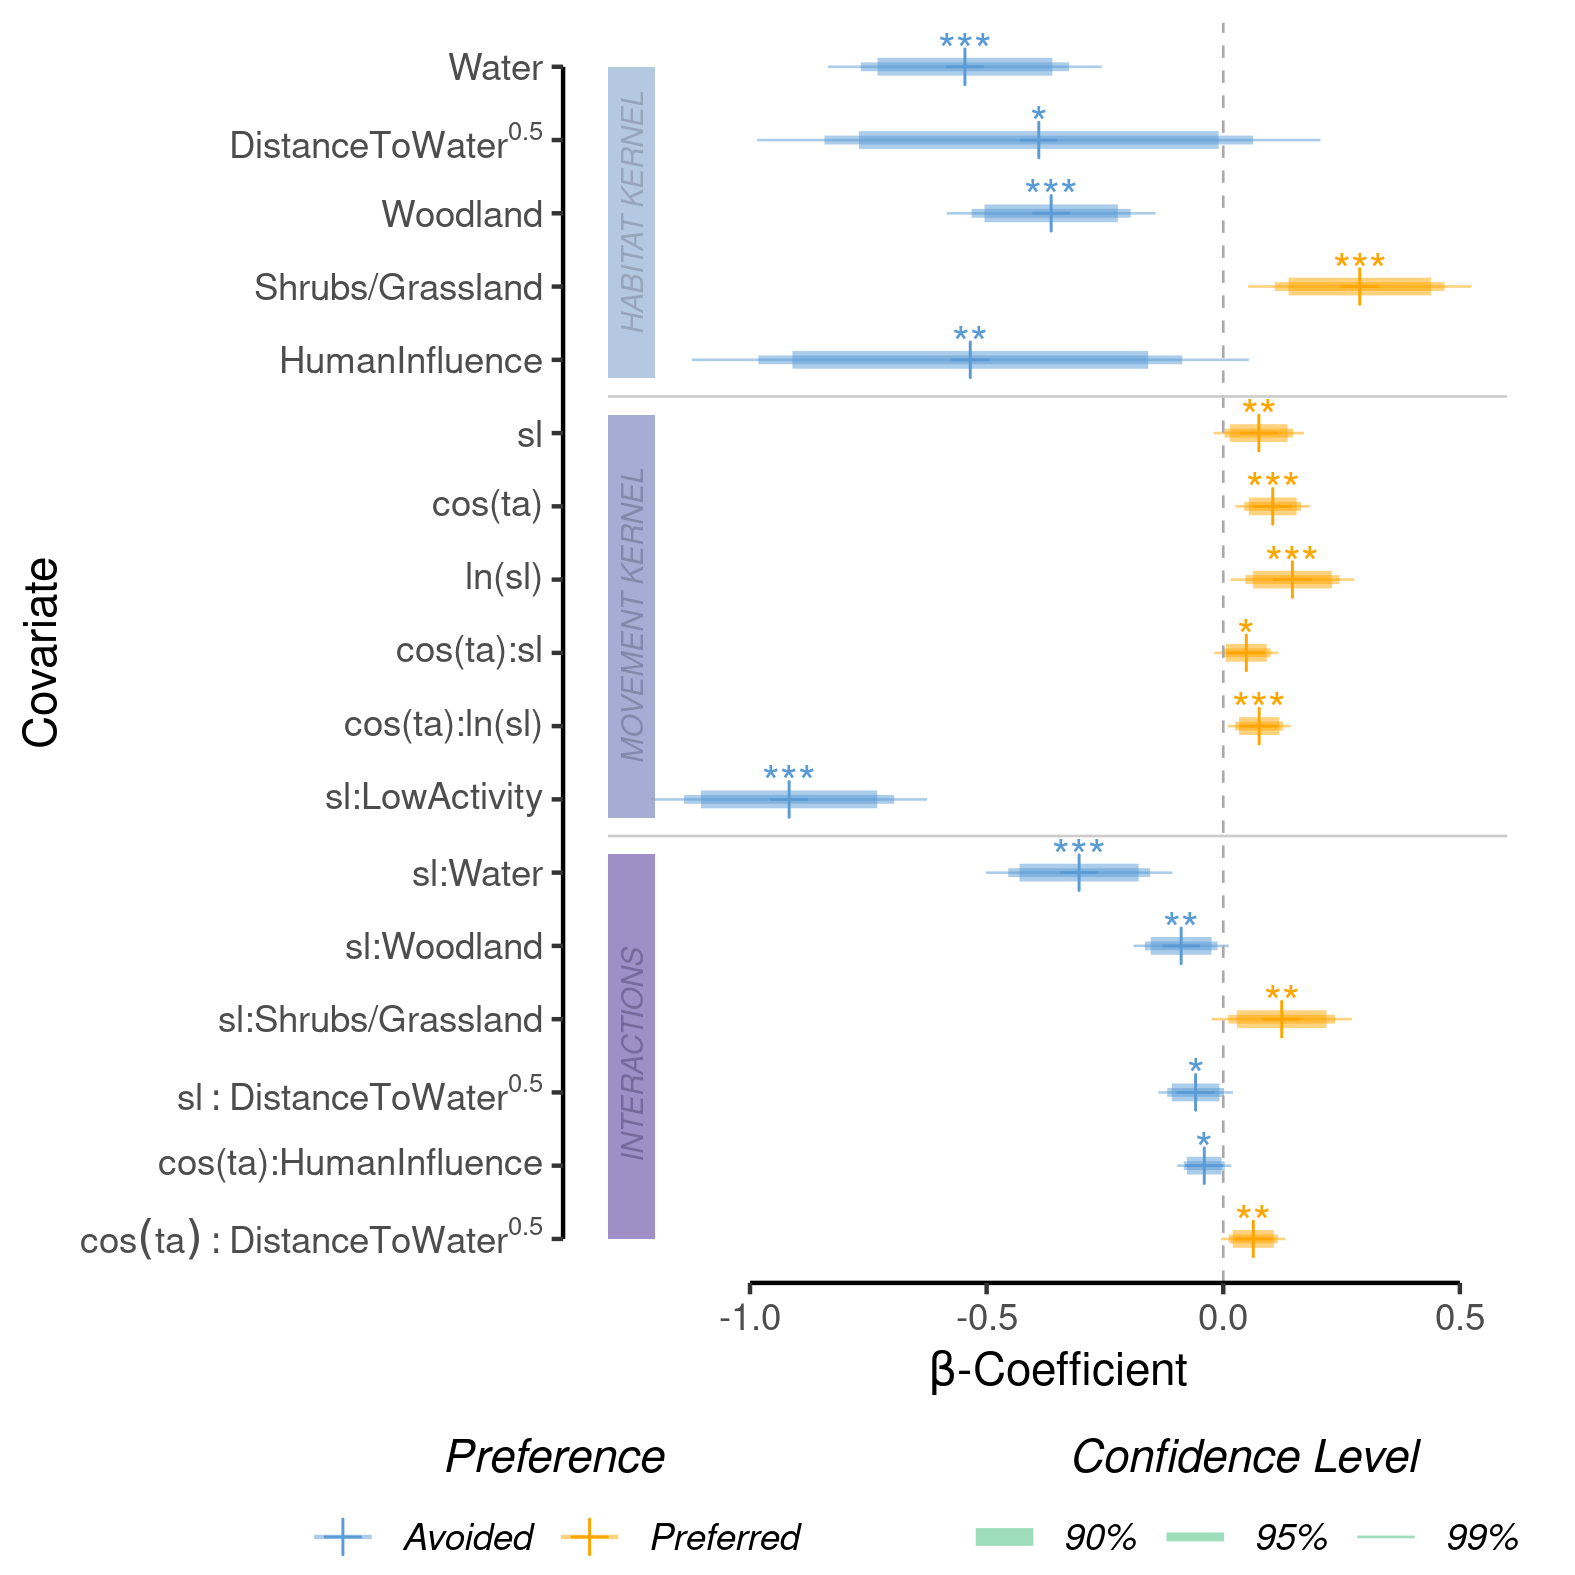
\includegraphics[width = \textwidth]{Figures/MovementModel.png}
  \caption{Model parameters from the step-selection model implemented by
  \citet{Hofmann.2023}. The model was fit to GPS data of dispersing African wild
  dogs and comprises of a habitat kernel (light blue band), a movement kernel
  (dark blue band), and their interactions (purple band). Abbreviations are as
  follows: sl = step-length, ln(sl) = natural logarithm of the step-length,
  cos(ta) = cosine of the relative turning angle.}
  \label{Model}
  \end{center}
\end{figure}

\newpage
\section{Immigration \& Emigration by Source Area}
\begin{figure}[htbp]
 \begin{center}
  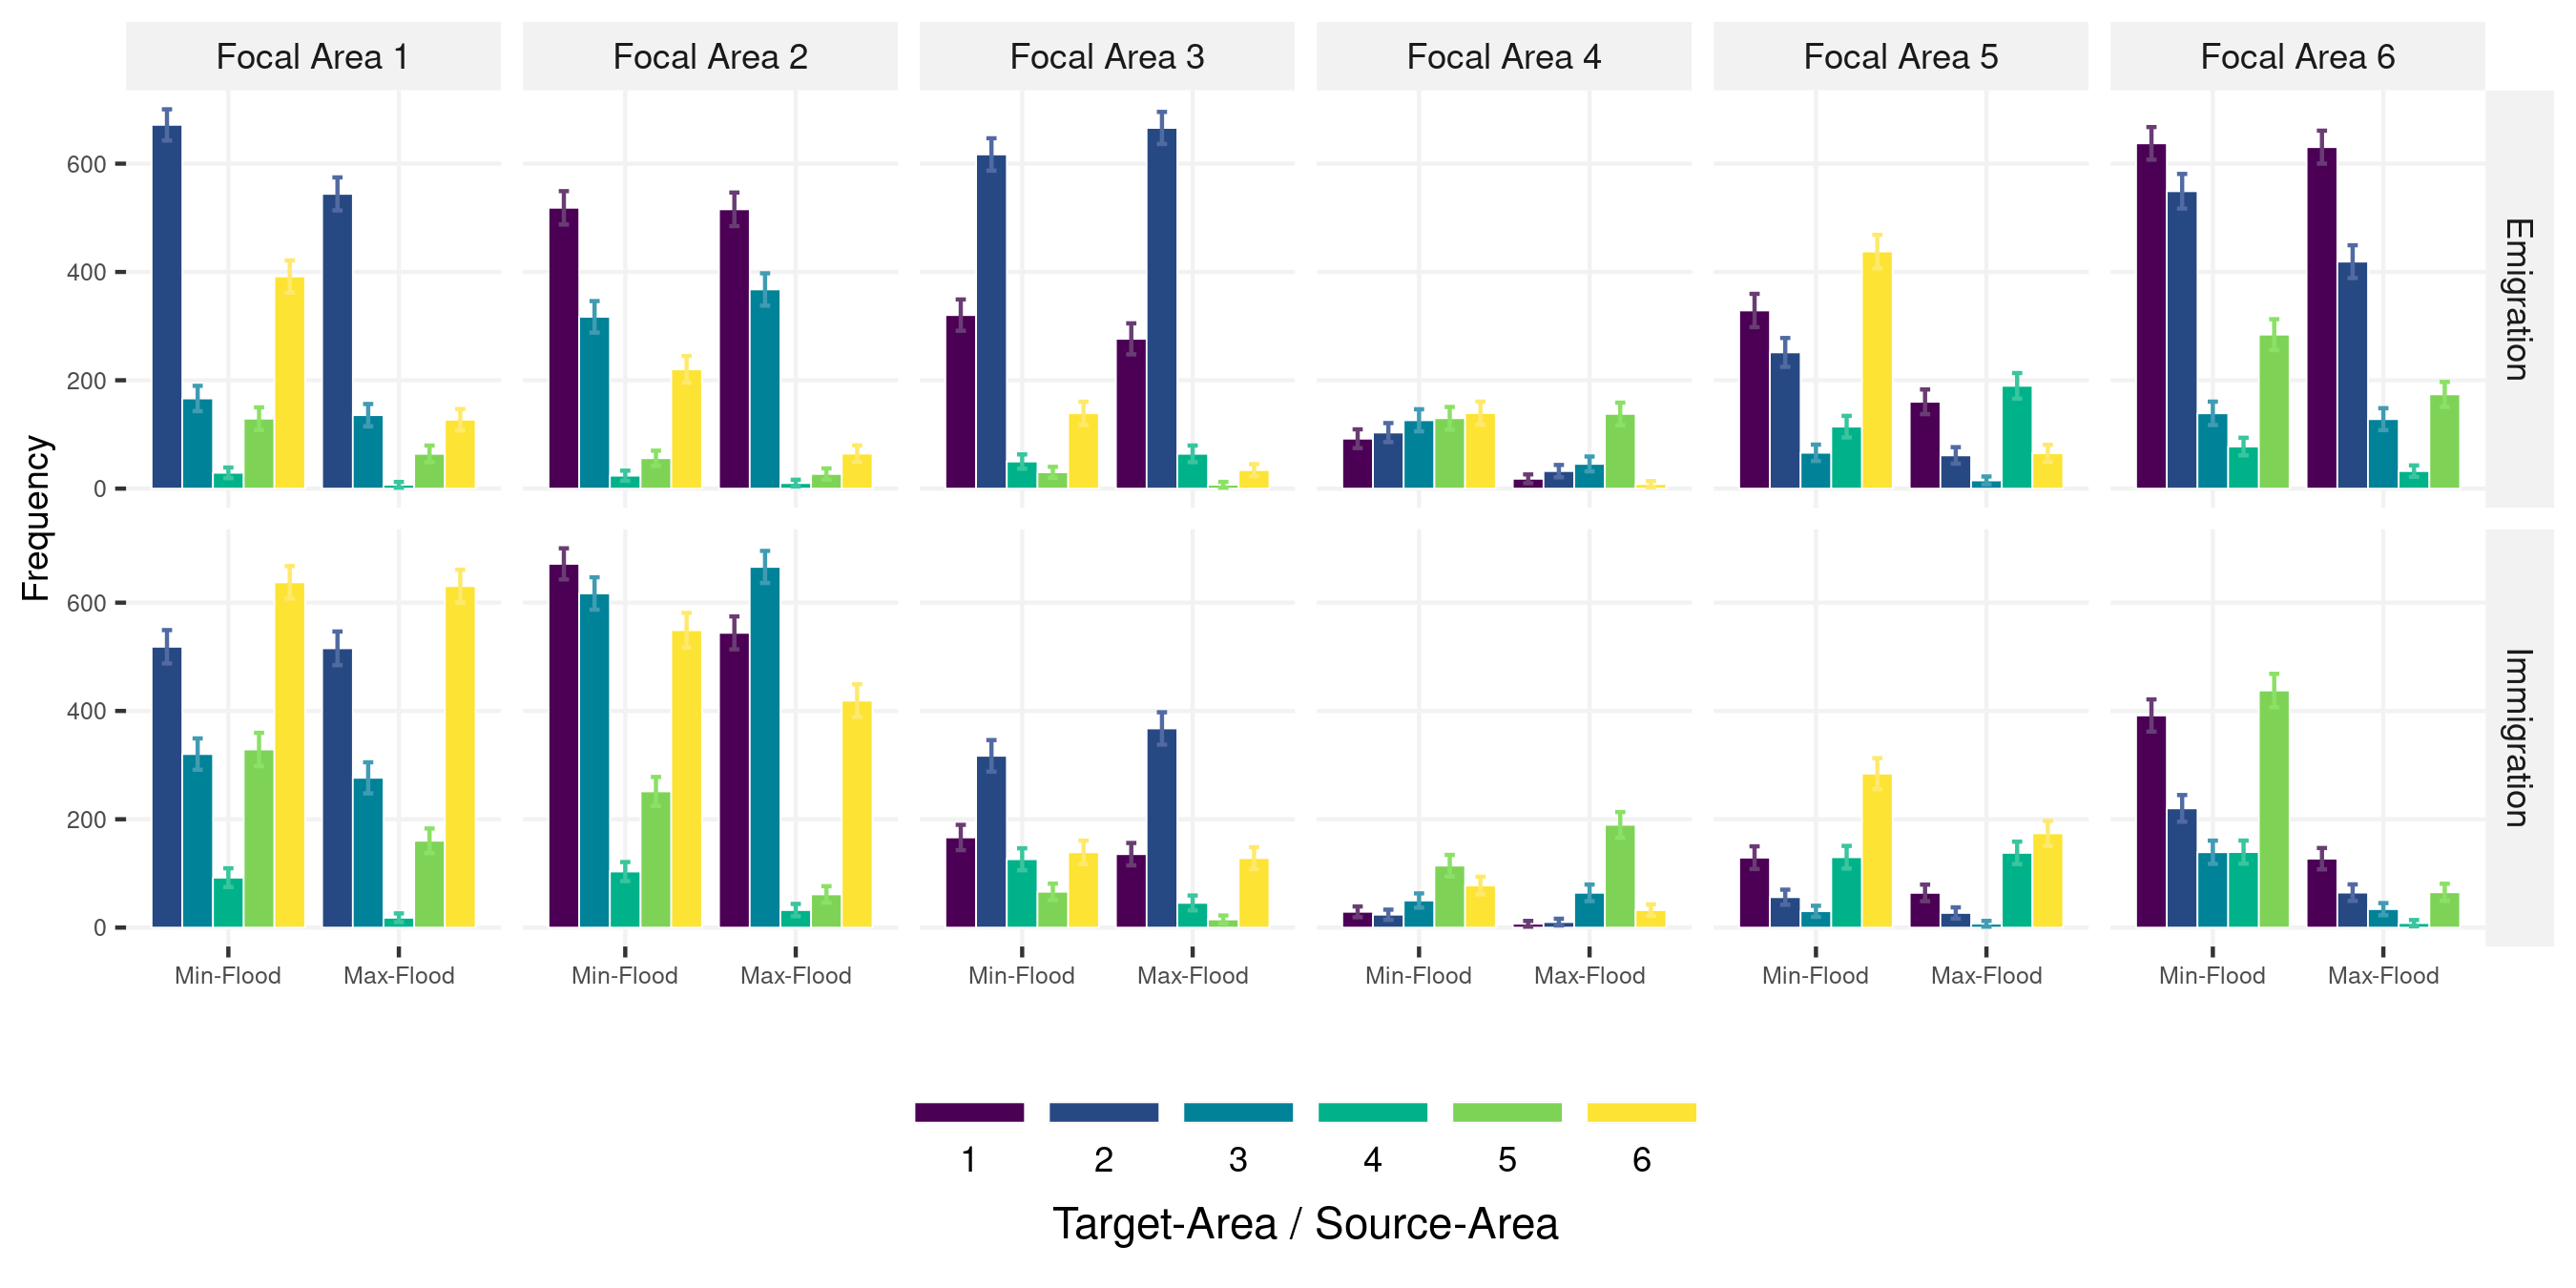
\includegraphics[width = \textwidth]{Figures/ImmigrationEmigration.png}
  \caption{Number of individuals emigrating from, or immigrating into a specific
  source area (focal area). Colors indicate into which other areas emigrants
  moved or from which other areas immigrants originate. For instance, the most
  left plot in the upper panel shows the number of individuals moving from
  source area 1 into the six other source areas during minimum and maximum
  flood, respectively.}
  \label{EmigrationImmigration}
 \end{center}
\end{figure}

\newpage
\section{Source-Specific Inter-Patch Connectivity}
\begin{figure}[htbp]
  \begin{center}
  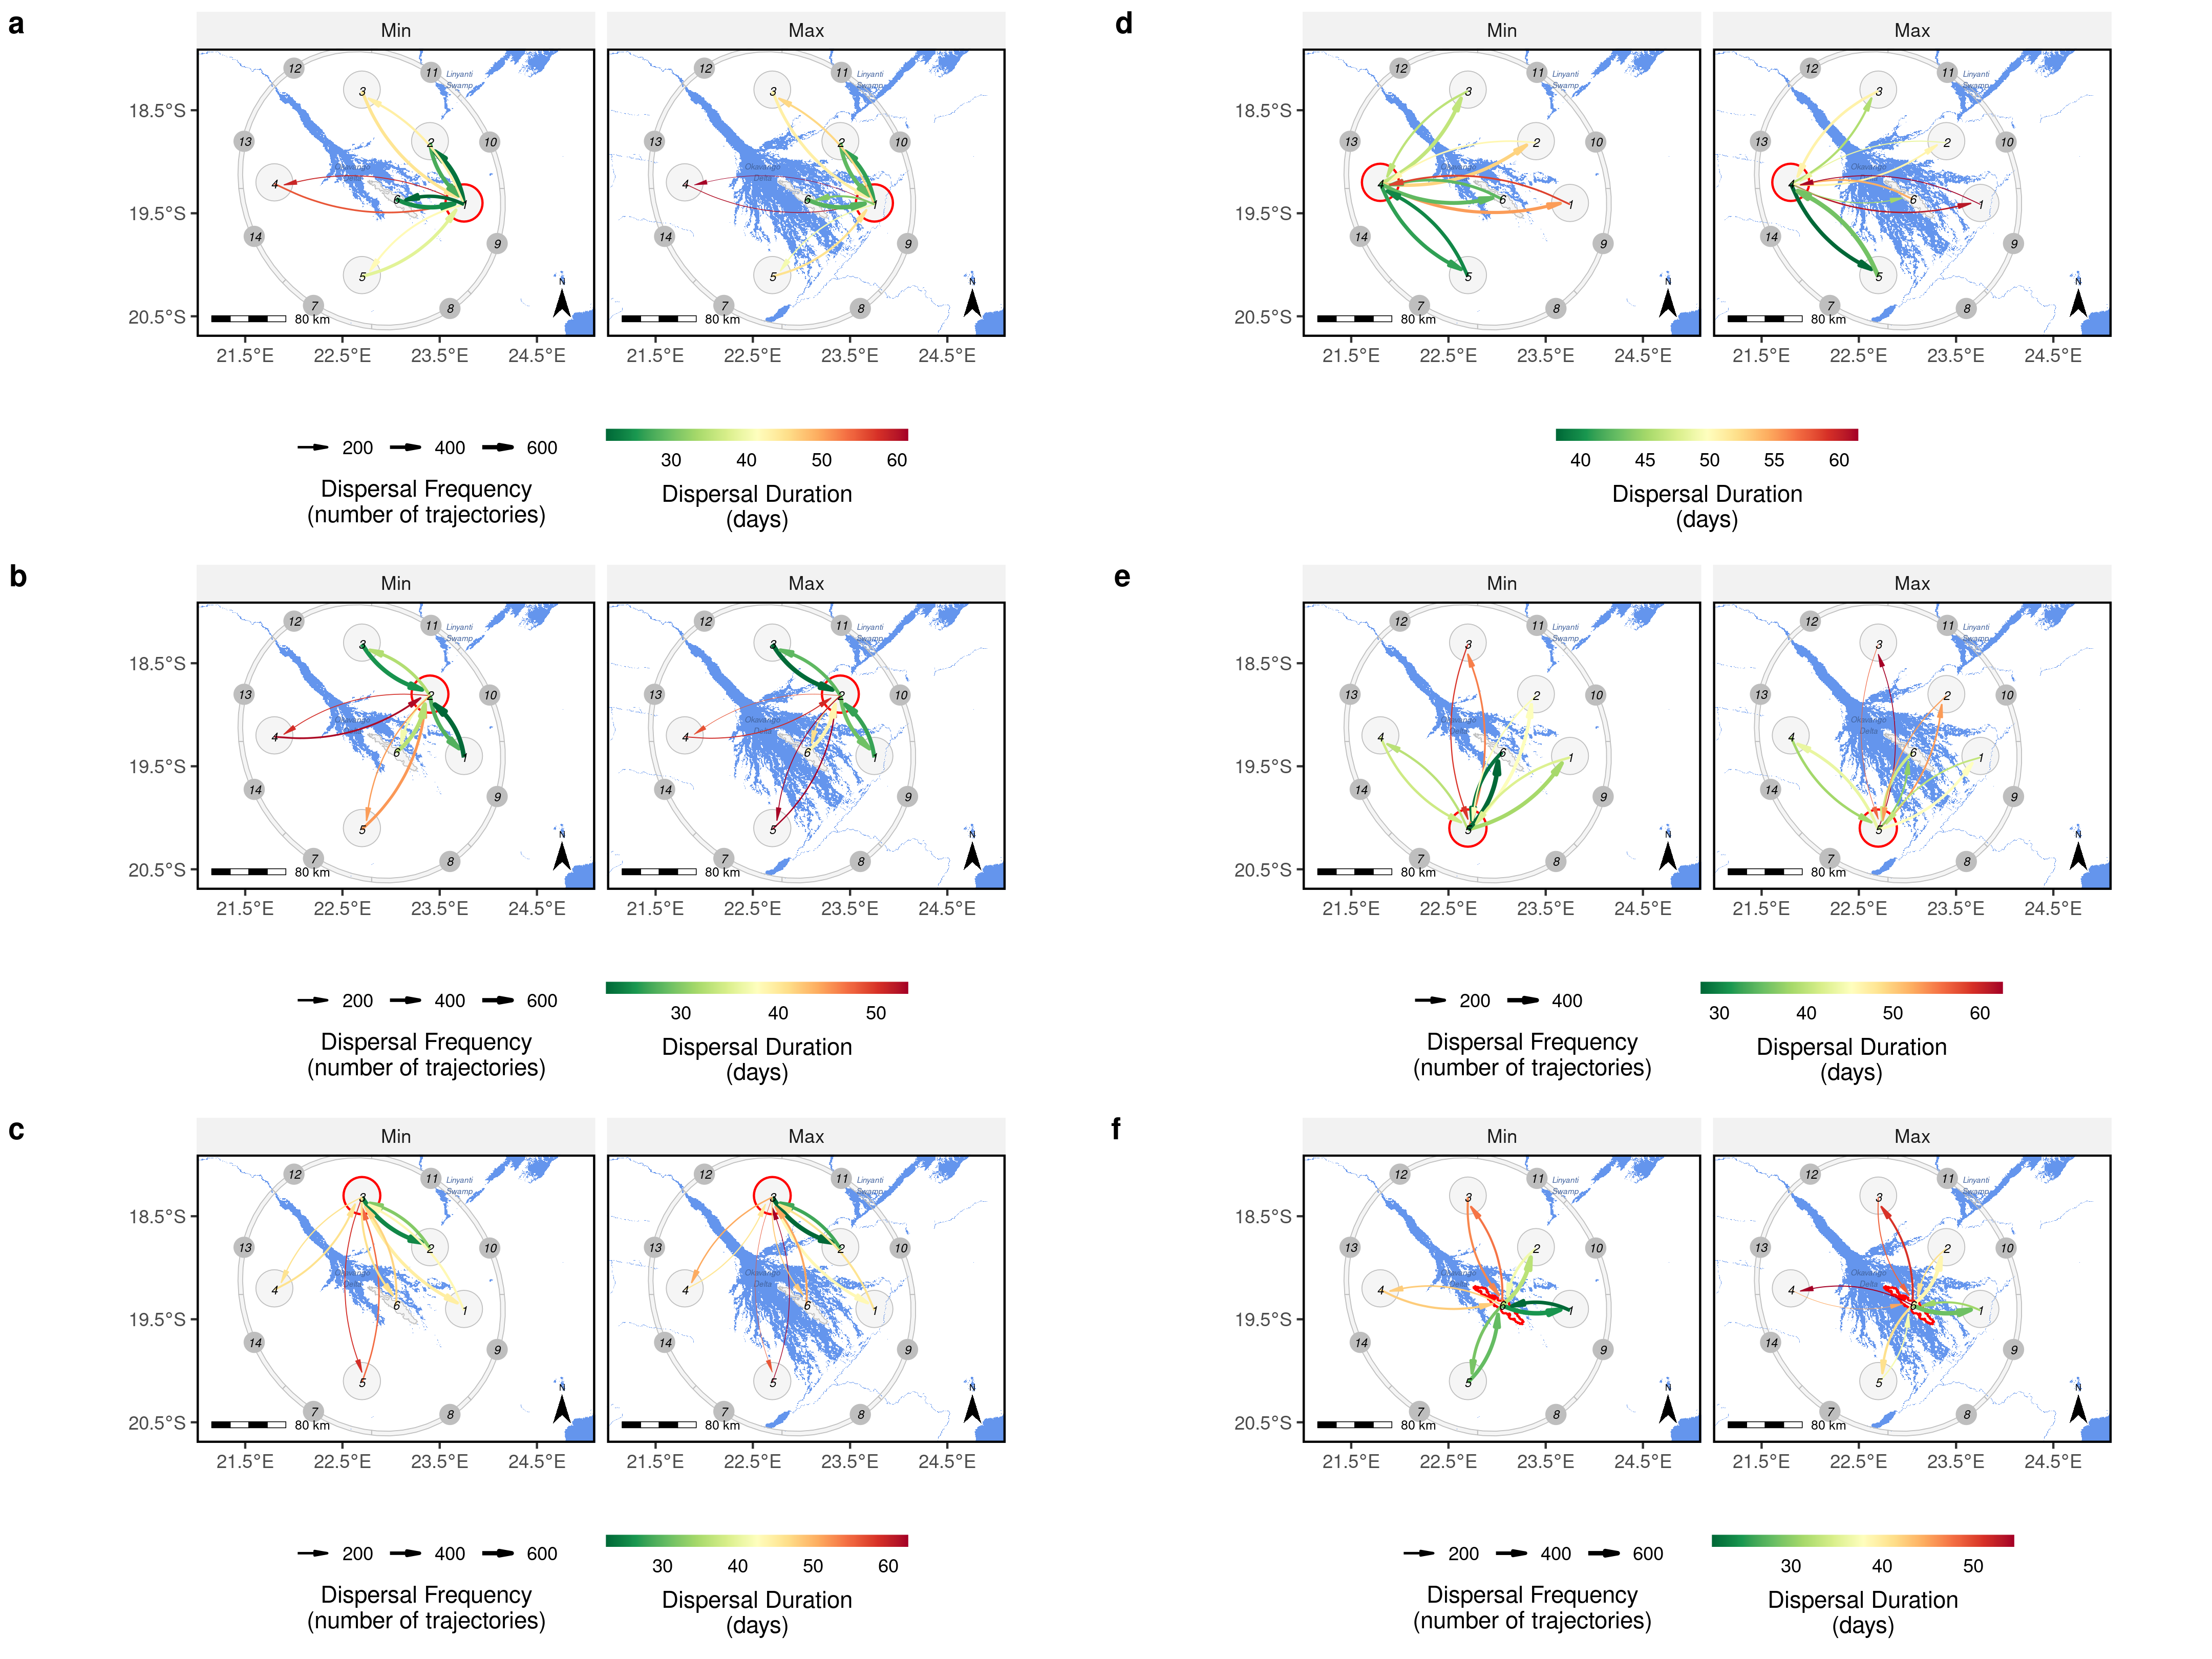
\includegraphics[width = \textwidth]{Figures/IPCMain.png}
  \caption{Spatial representation of inter-patch connectivity derived for each
  source area separately across the two extreme flood-scenarios. The focal
  source area of each subfigure is highlighted by a red circle. Subfigure (a),
  for instance, depicts inter-patch connectivity for source area 1.}
  \label{IPCMain}
  \end{center}
\end{figure}

\newpage
\begin{figure}[htbp]
  \begin{center}
  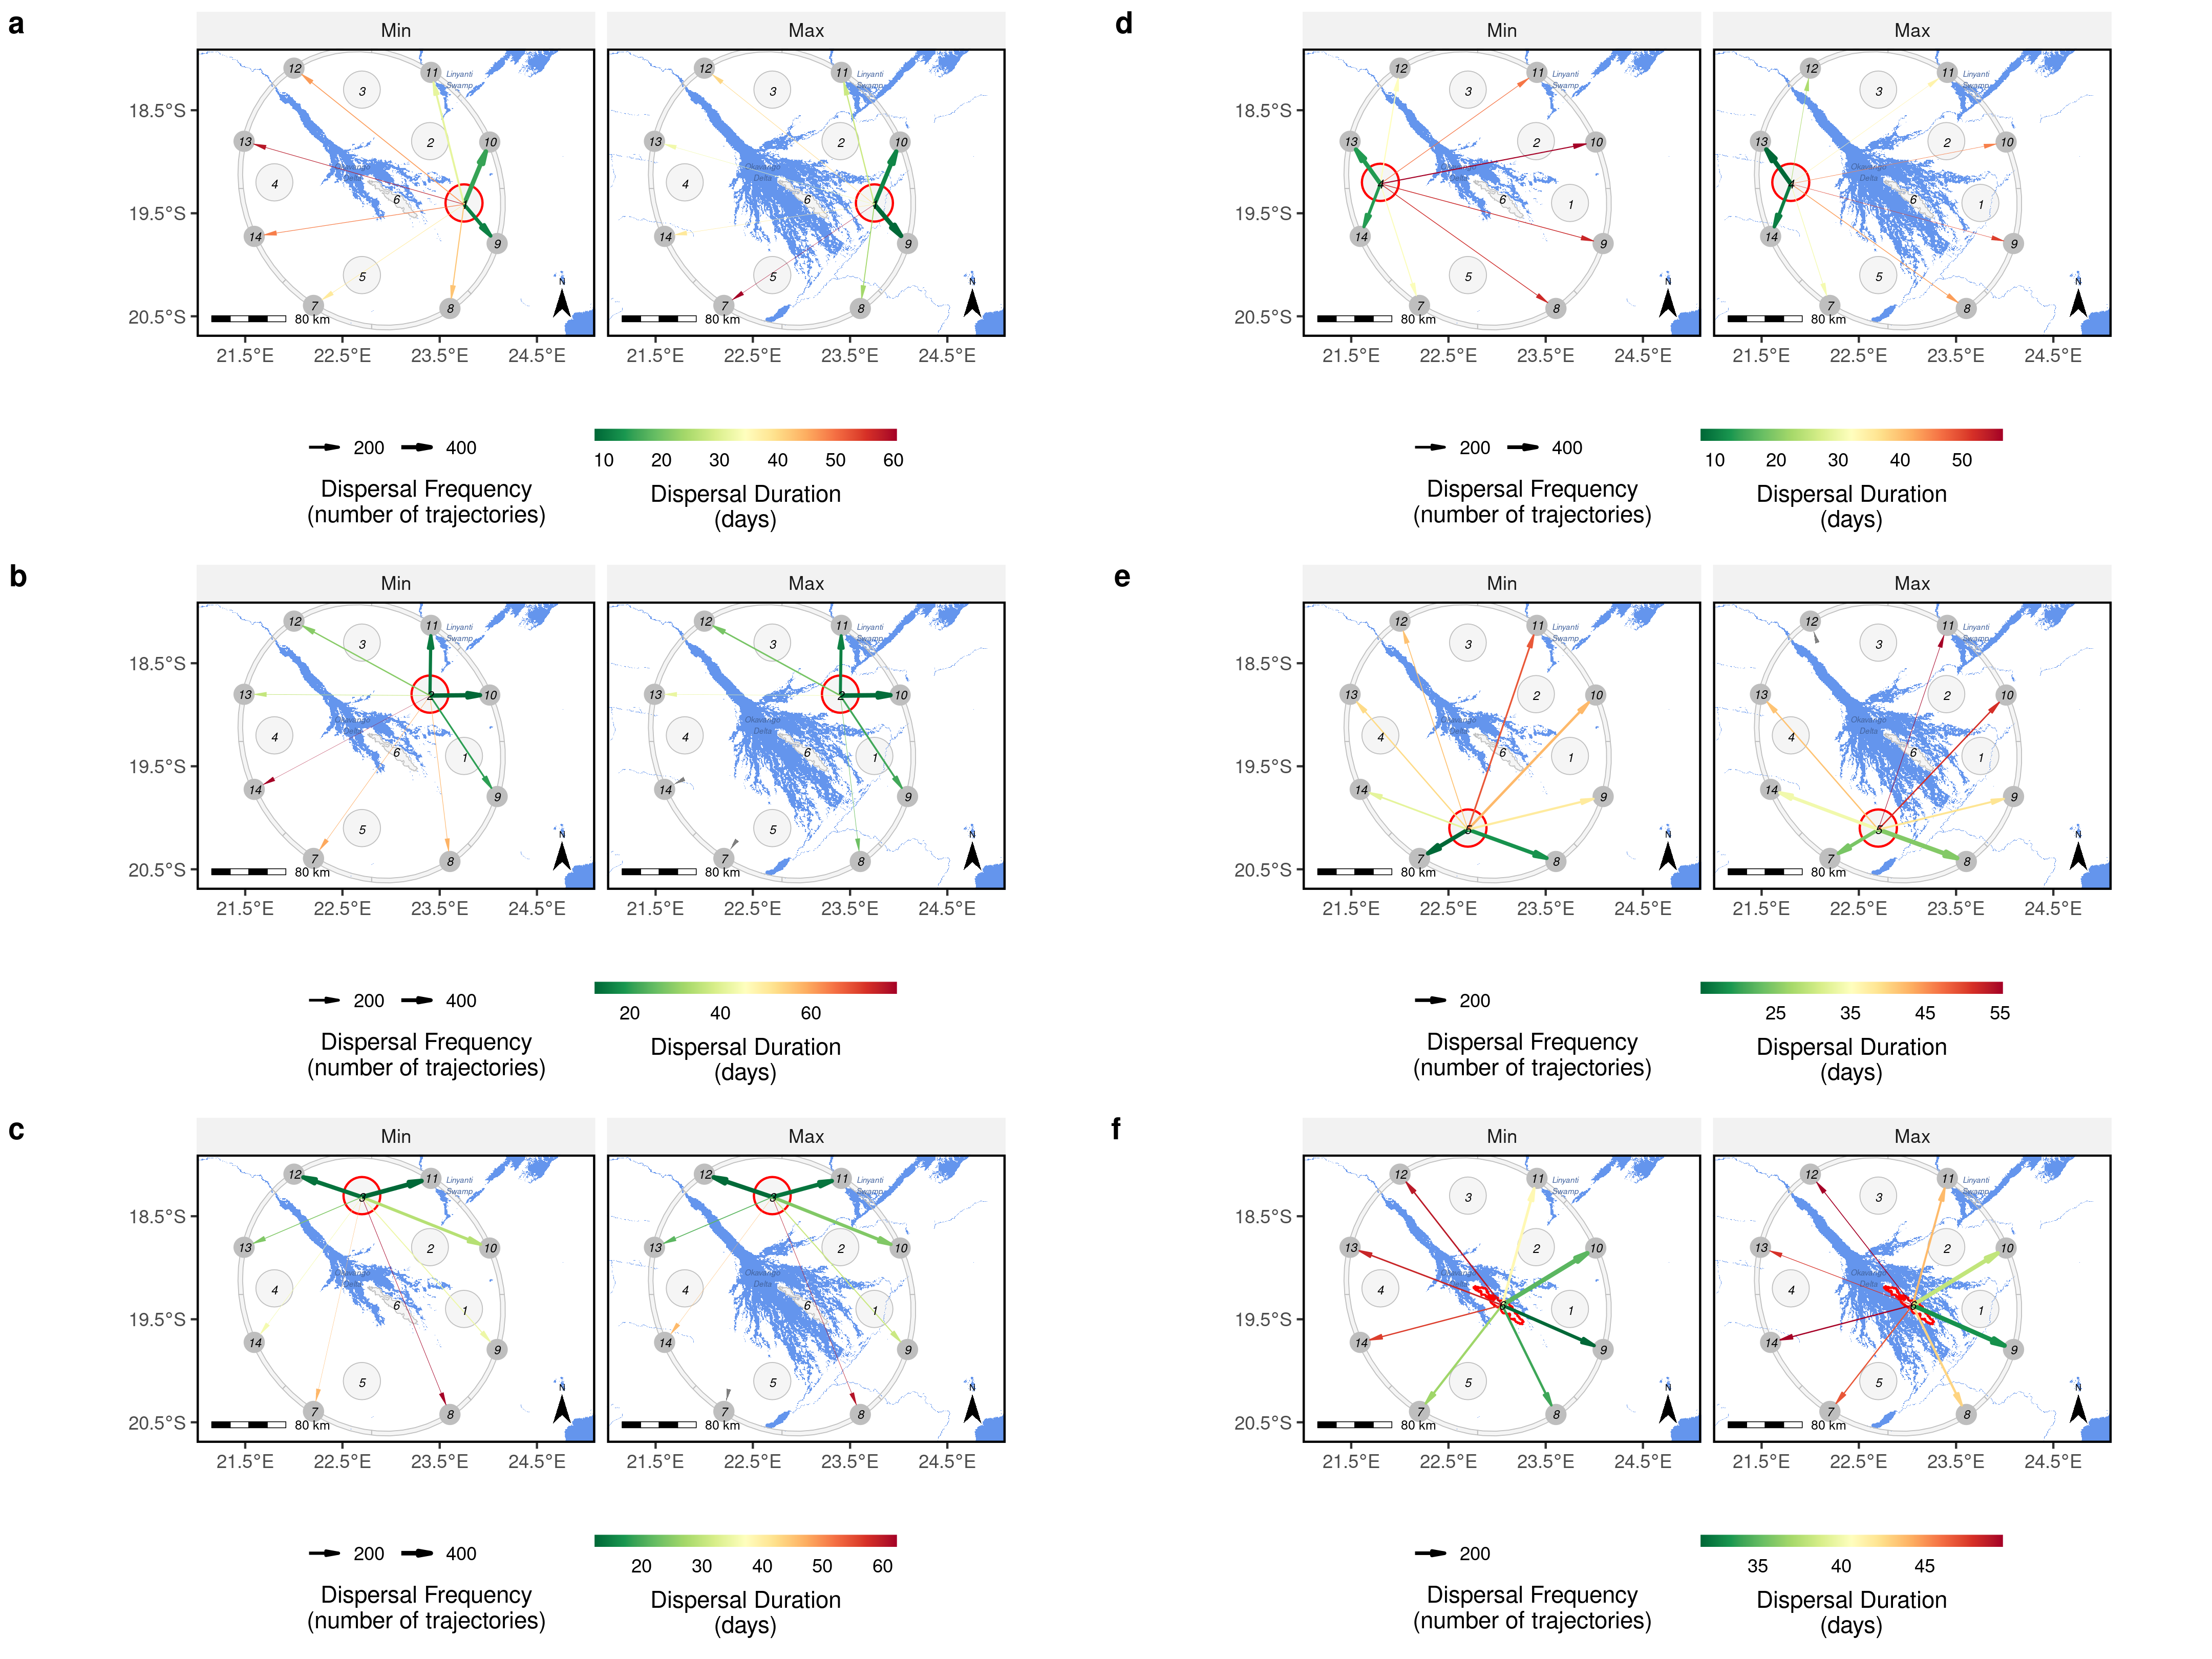
\includegraphics[width = \textwidth]{Figures/IPCBuffer.png}
  \caption{Spatial representation of egression patterns derived for each
  source area separately across the two extreme flood-scenarios. The focal
  source area of each subfigure is highlighted by a red circle. Subfigure (a),
  for instance, depicts the number of individuals egressing from source area
  1.}
  \label{IPCBuffer}
  \end{center}
\end{figure}

\newpage
\section{Dispersal into Egression Zones}
\begin{figure}[htbp]
  \begin{center}
  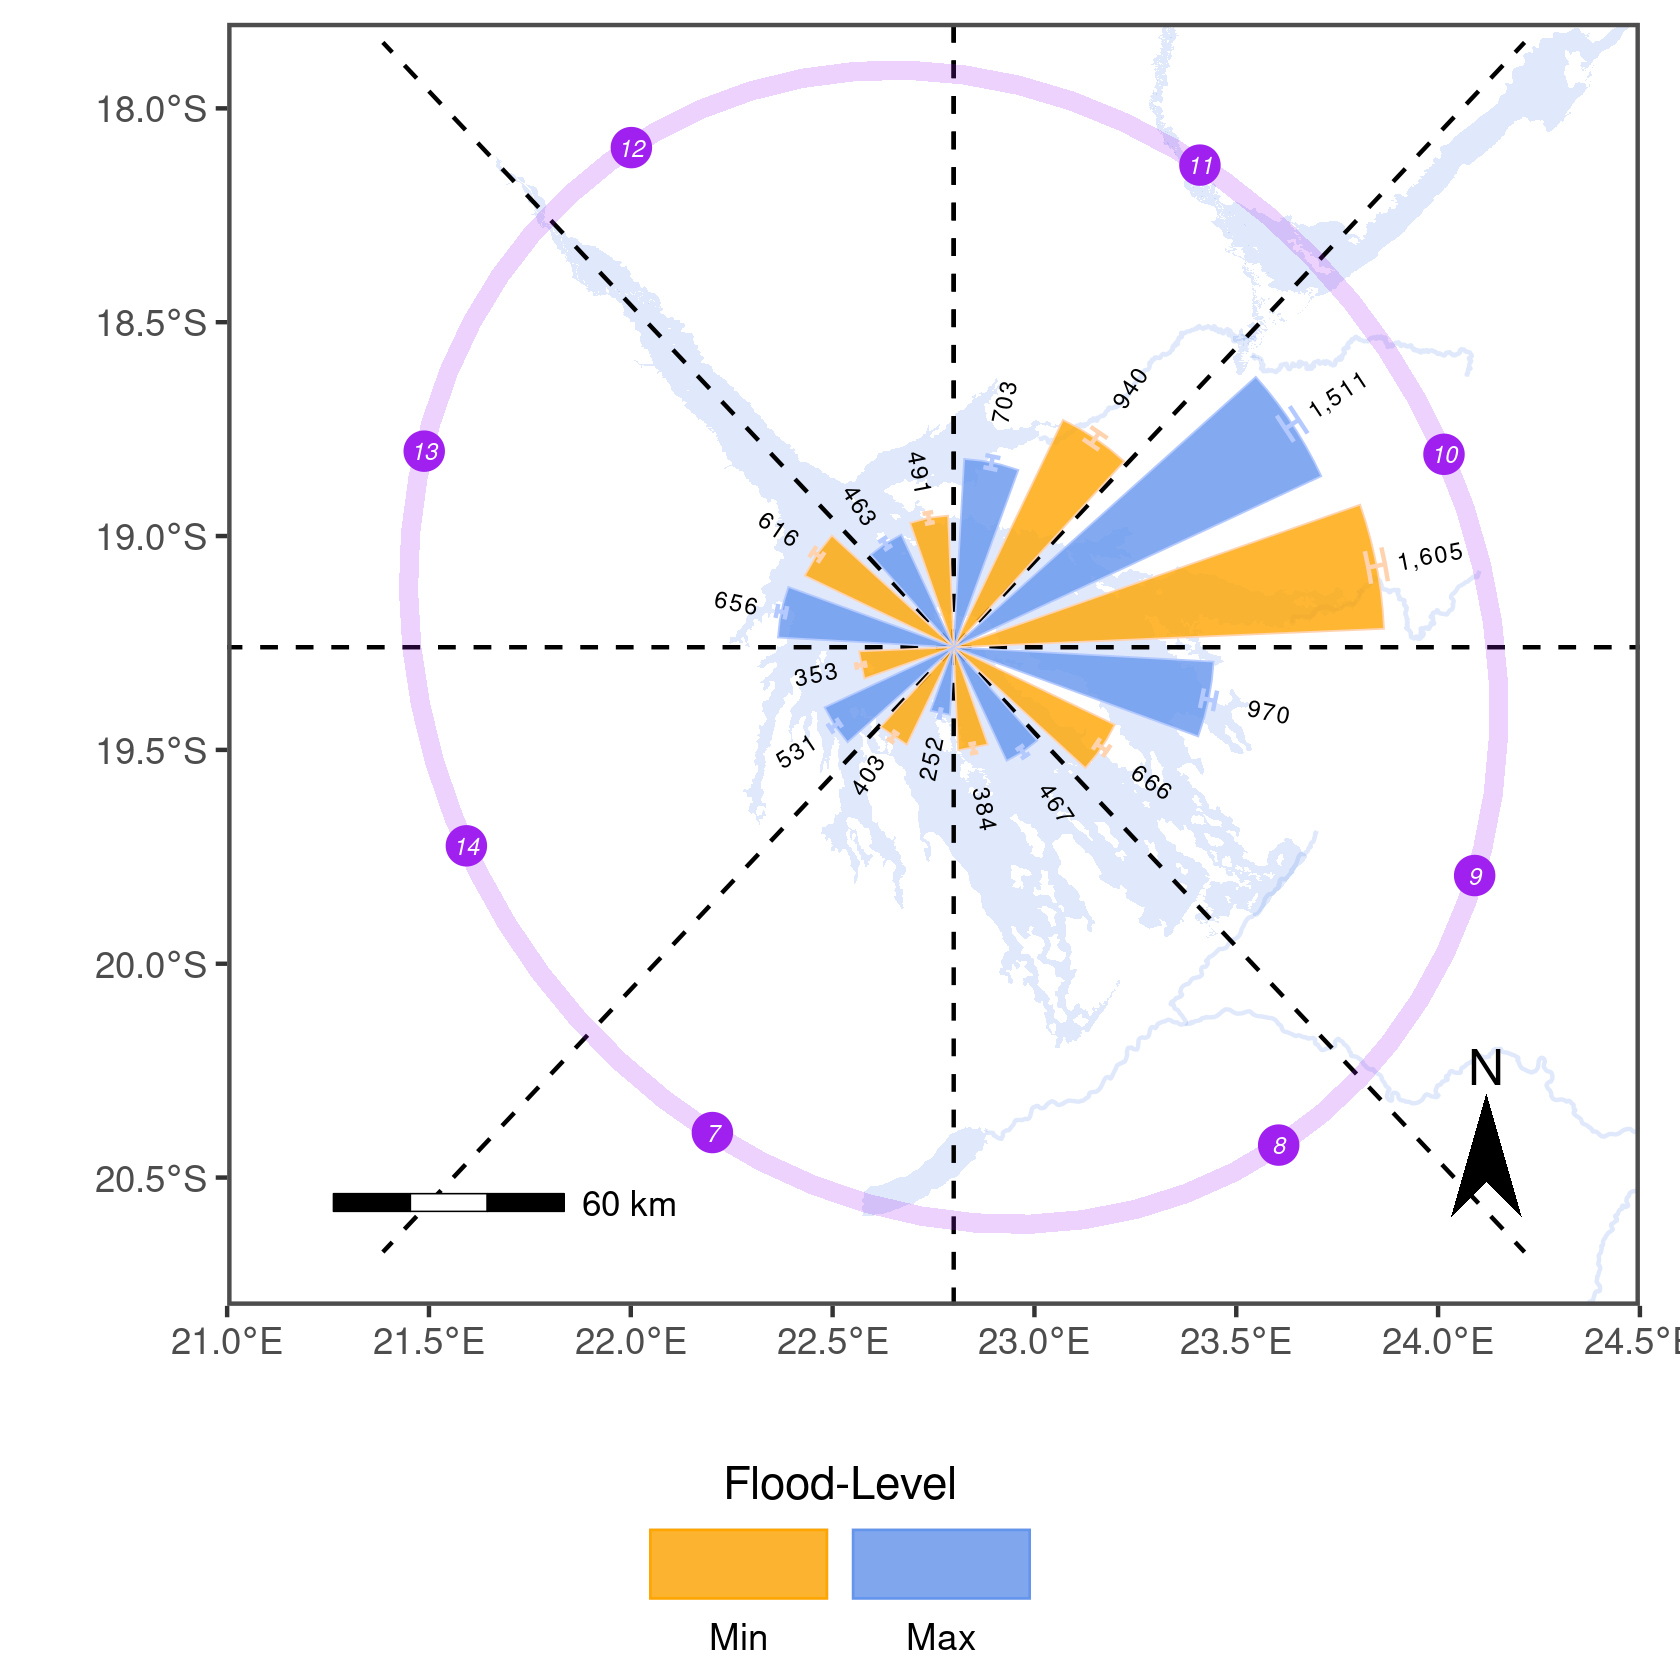
\includegraphics[width = \textwidth]{Figures/Egression.png}
  \caption{Absolute number of simulated trajectories running into each of the
  designated egression zones (purple) during minimum and maximum flood.}
  \label{Egression}
  \end{center}
\end{figure}

\newpage
\section{Source-Specific Intensity of Use}
\begin{figure}[htbp]
  \begin{center}
  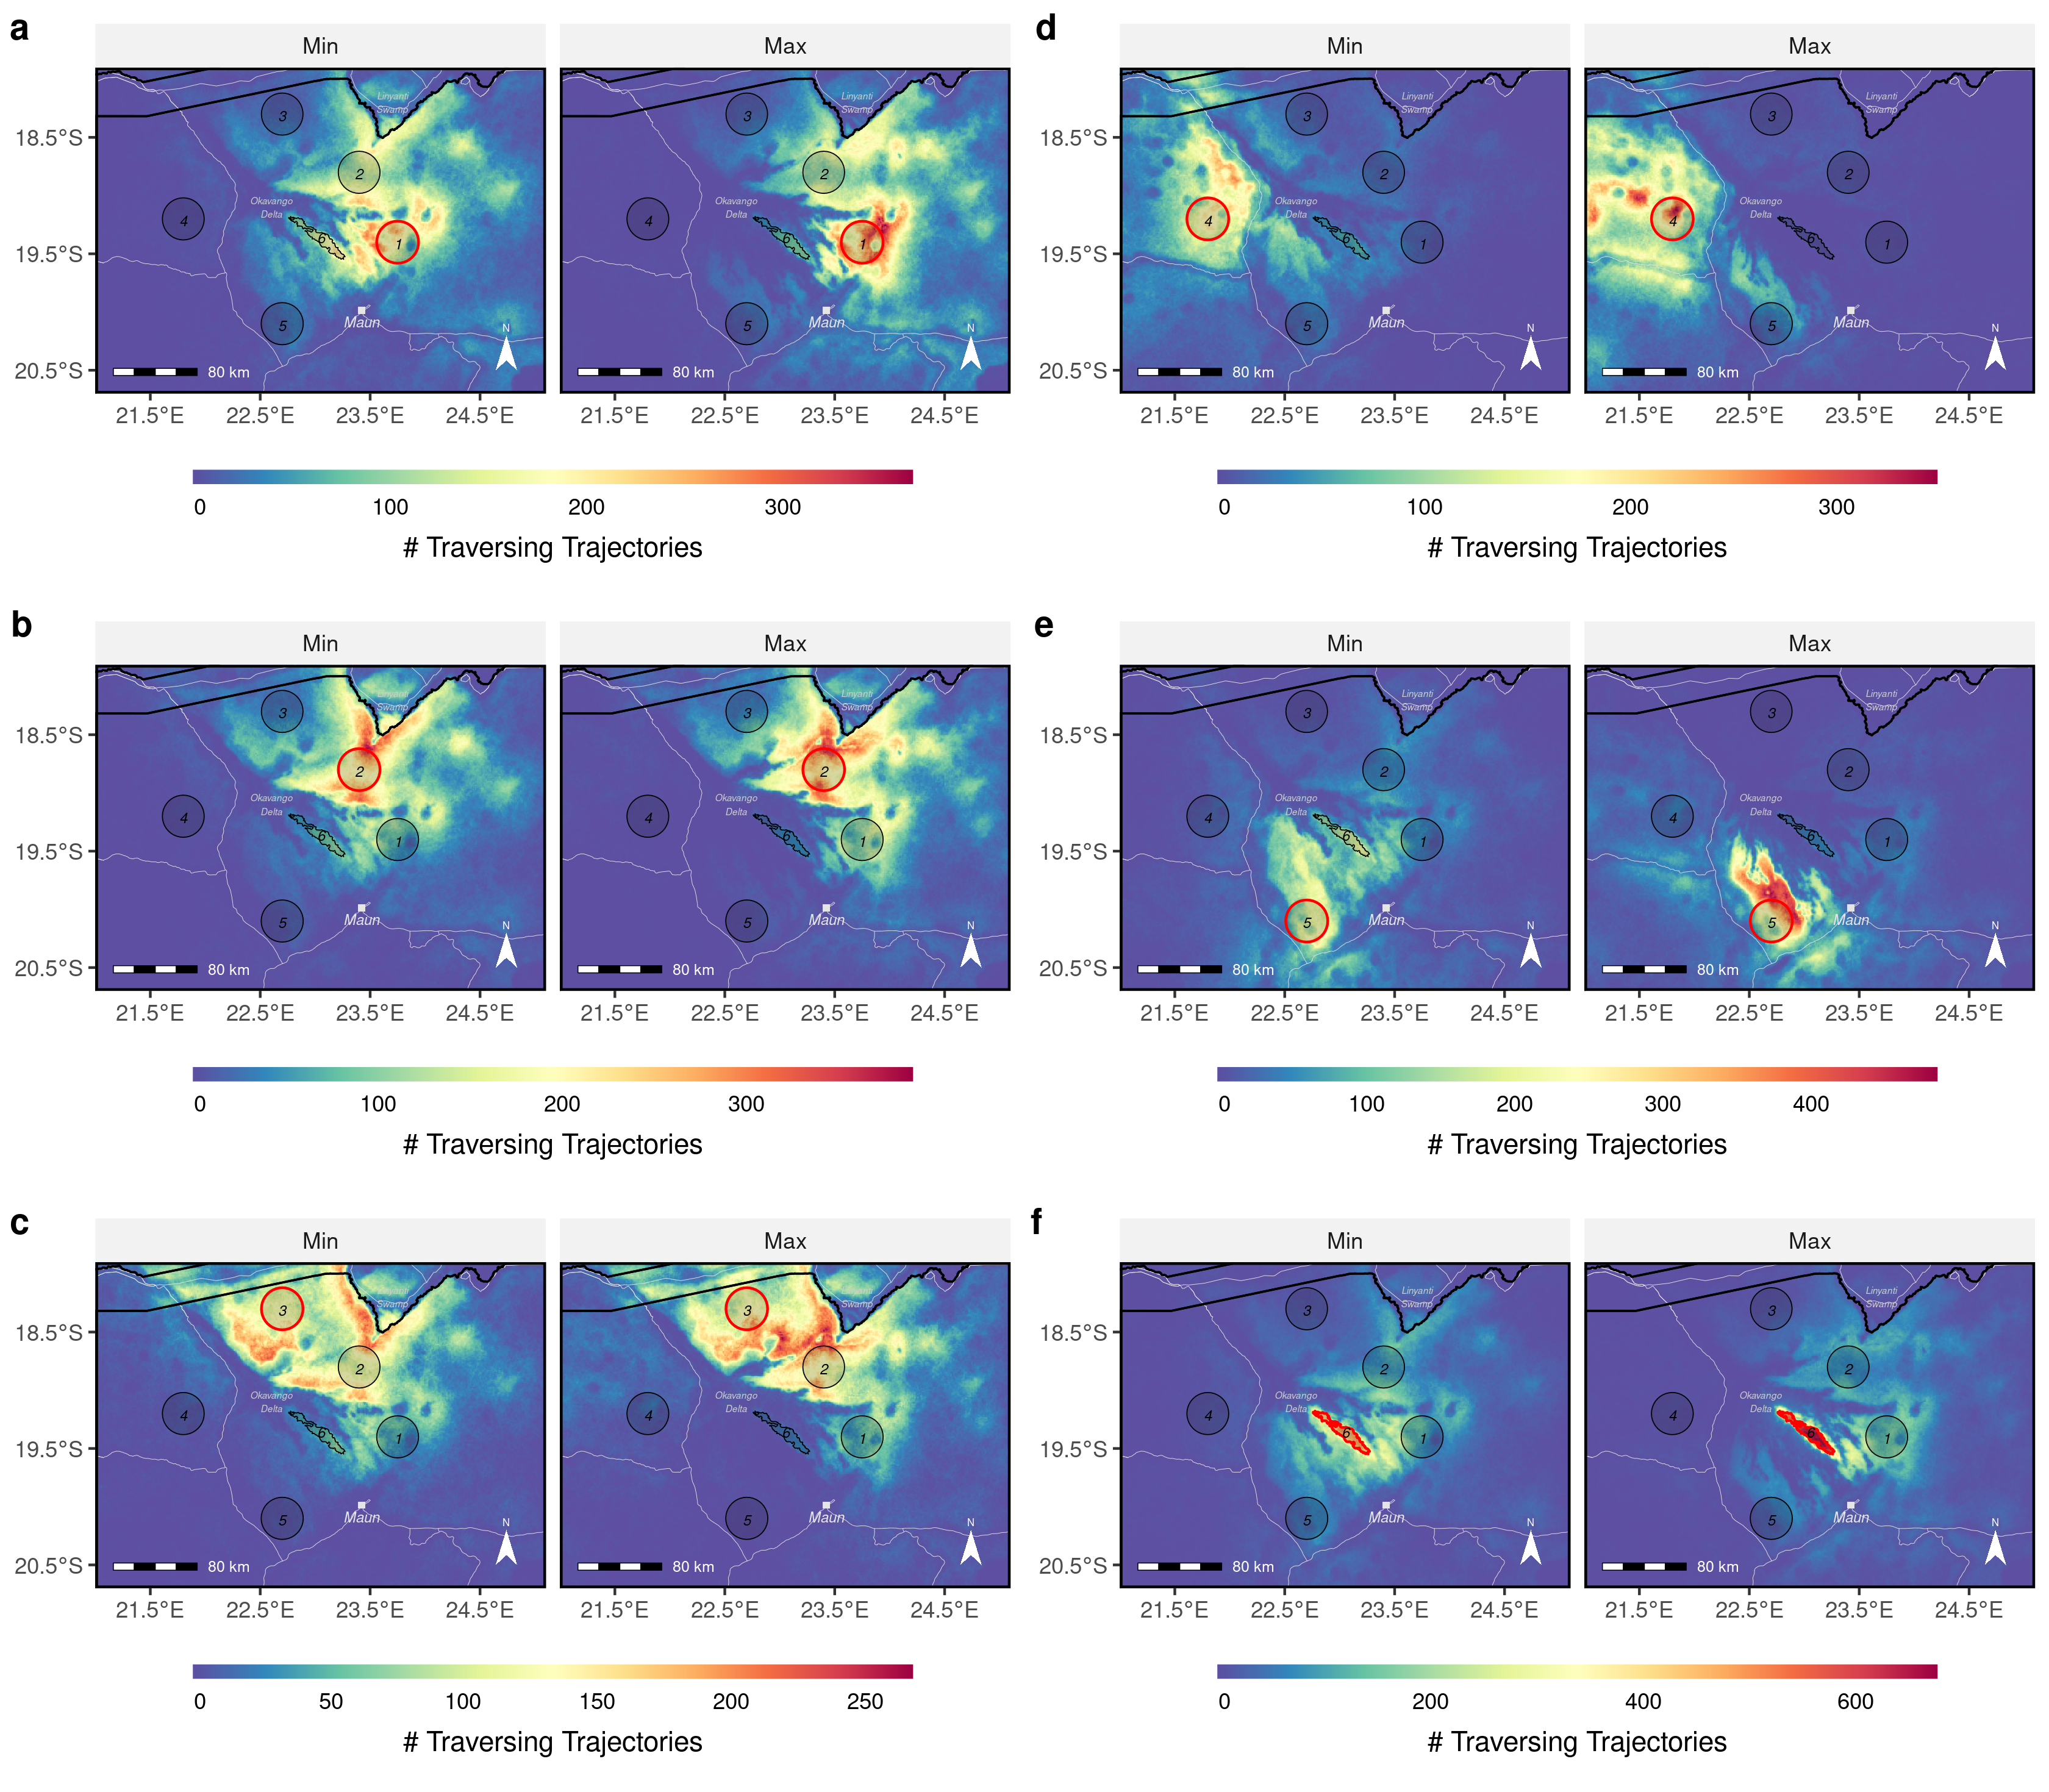
\includegraphics[width = \textwidth]{Figures/HeatmapsIndividual.png}
  \caption{Heatmaps showing the intensity of use for each source area separately
  across the two extreme flood-scenarios. The focal source area of each
  subfigure is highlighted by a red circle. Subfigure (a), for instance, depicts
  the heatmaps for source area 1.}
  \label{Heatmaps}
  \end{center}
\end{figure}

\newpage
\section{Source-Specific Betweenness}
\begin{figure}[htbp]
  \begin{center}
  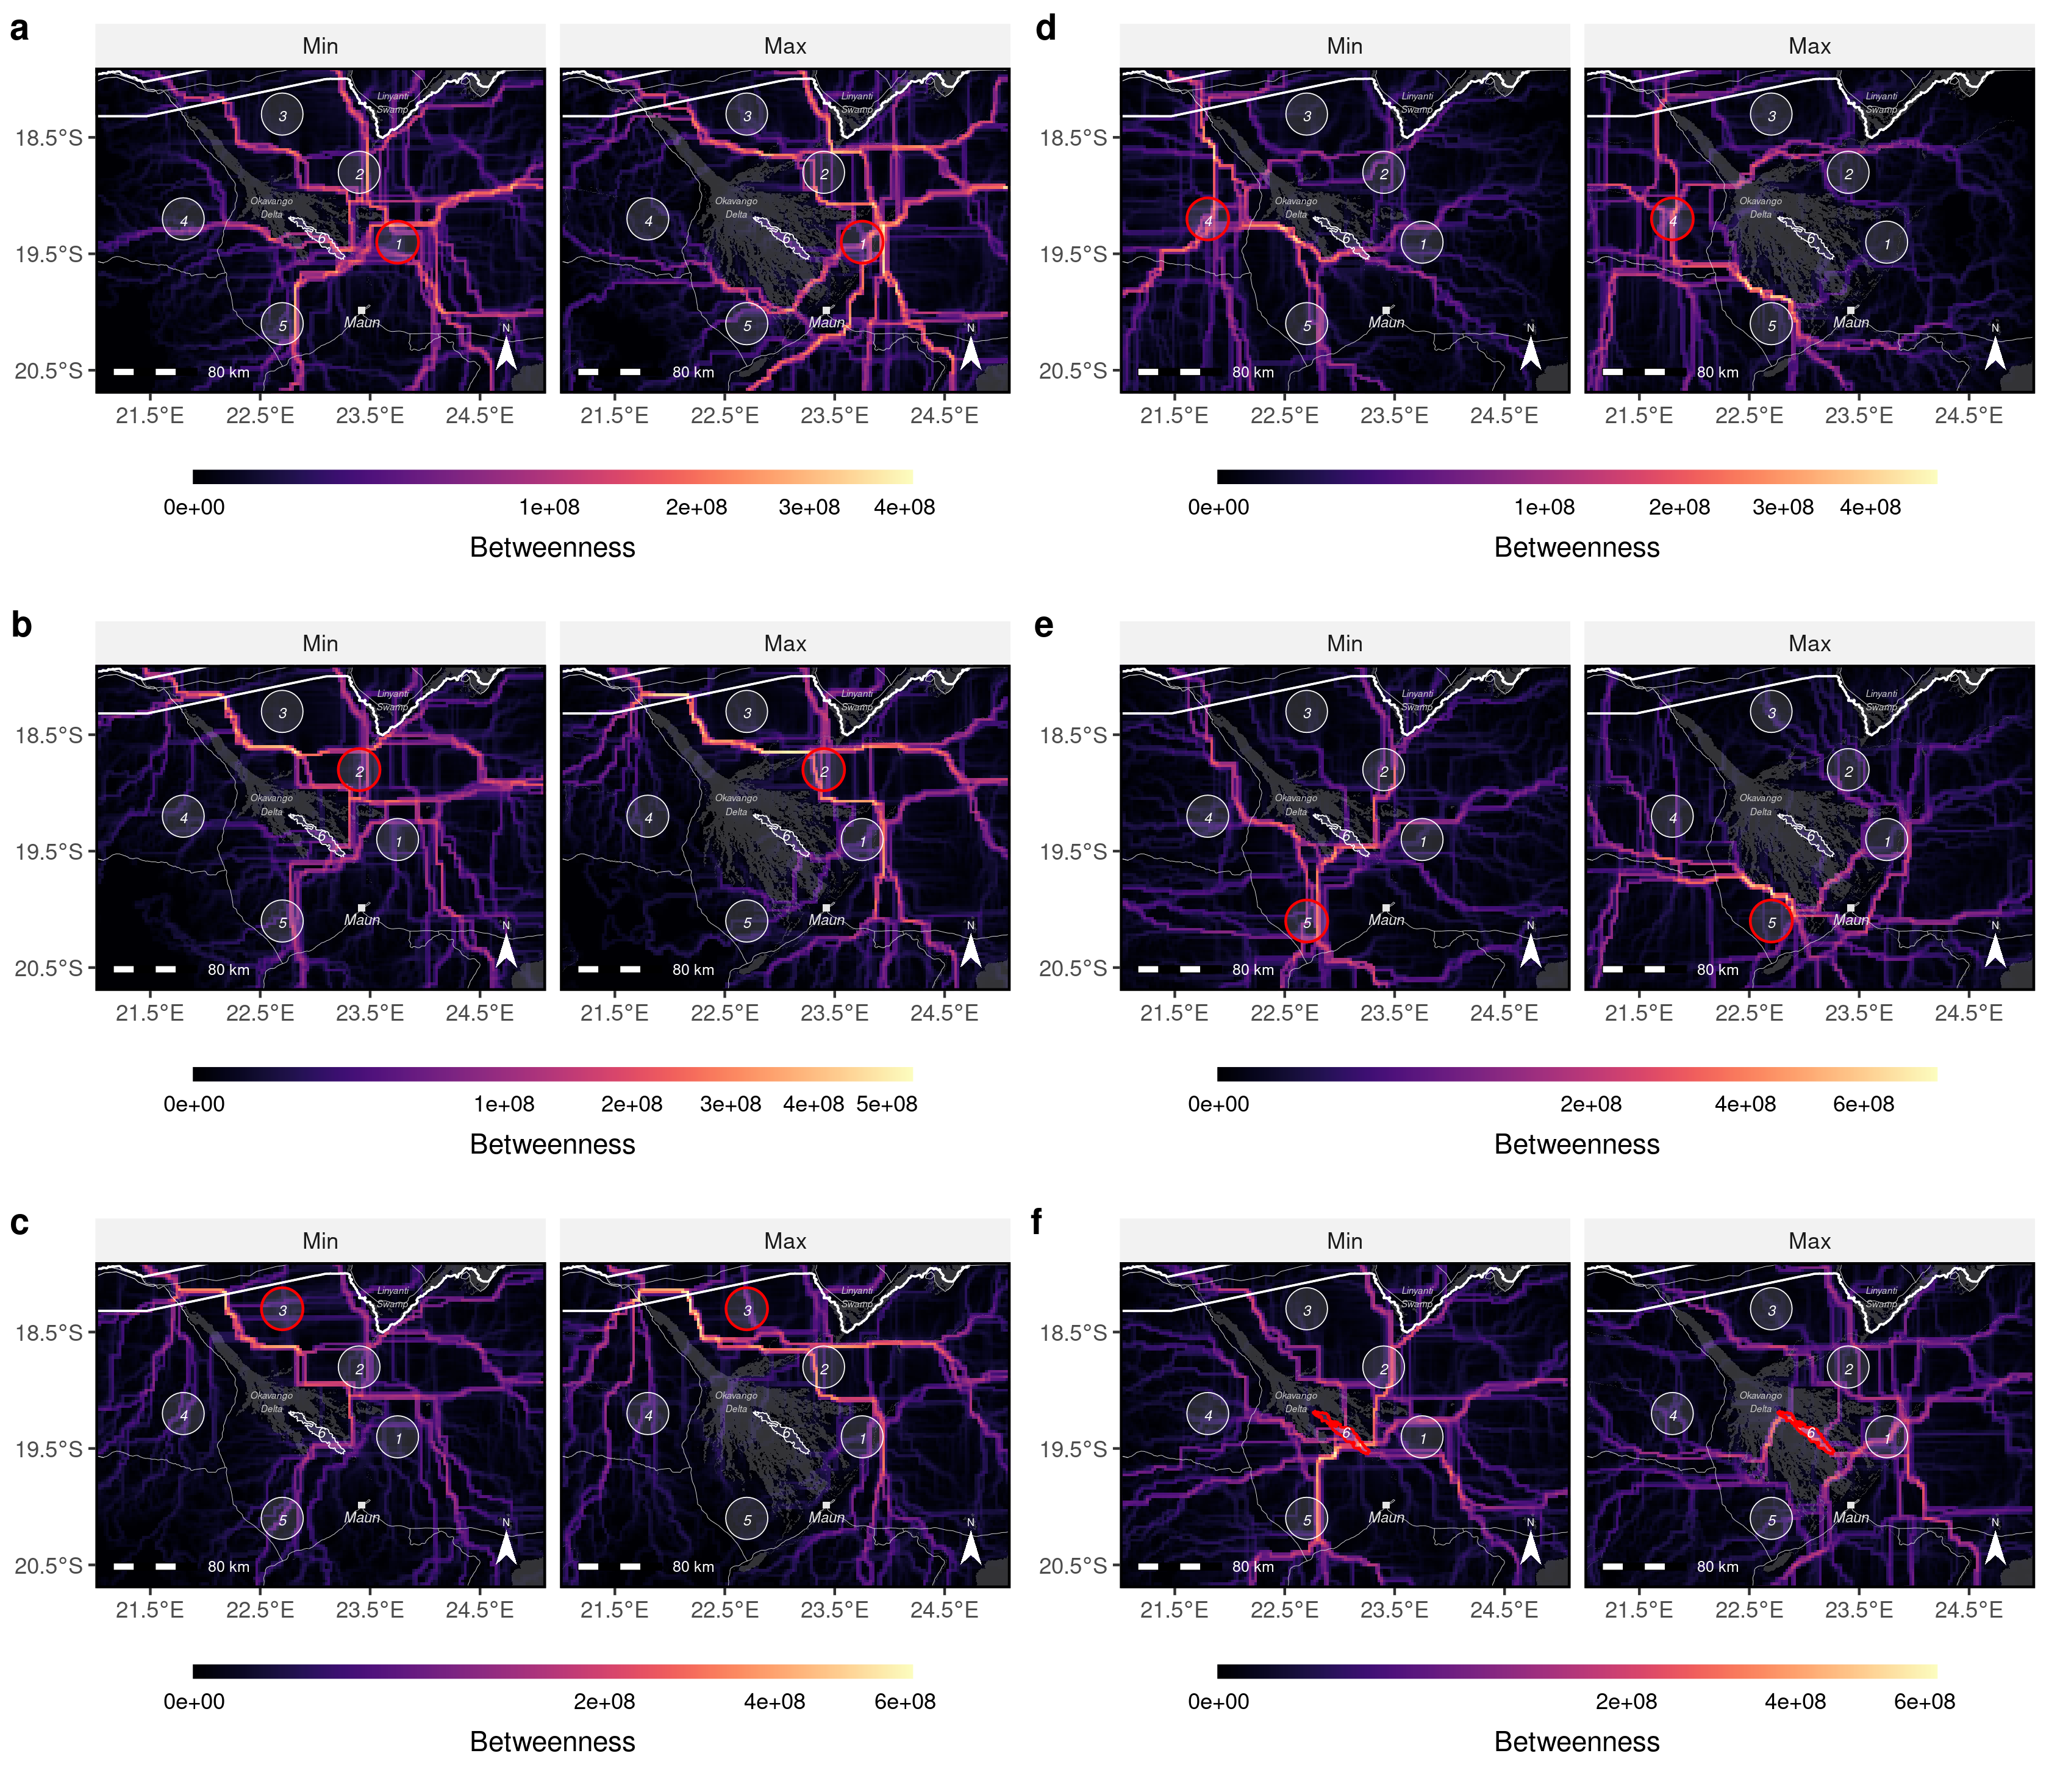
\includegraphics[width = \textwidth]{Figures/BetweennessIndividual.png}
  \caption{Betweenness maps prepared for each source area separately across the
  two extreme flood-scenarios. The focal source area of each subfigure is
  highlighted by a red circle. Subfigure (a), for instance, depicts the
  betweenness maps for source area 1.}
  \label{Betweenness}
  \end{center}
\end{figure}

\newpage
\section{Source-Specific Human-Wildlife Conflict}
\begin{figure}[htbp]
  \begin{center}
  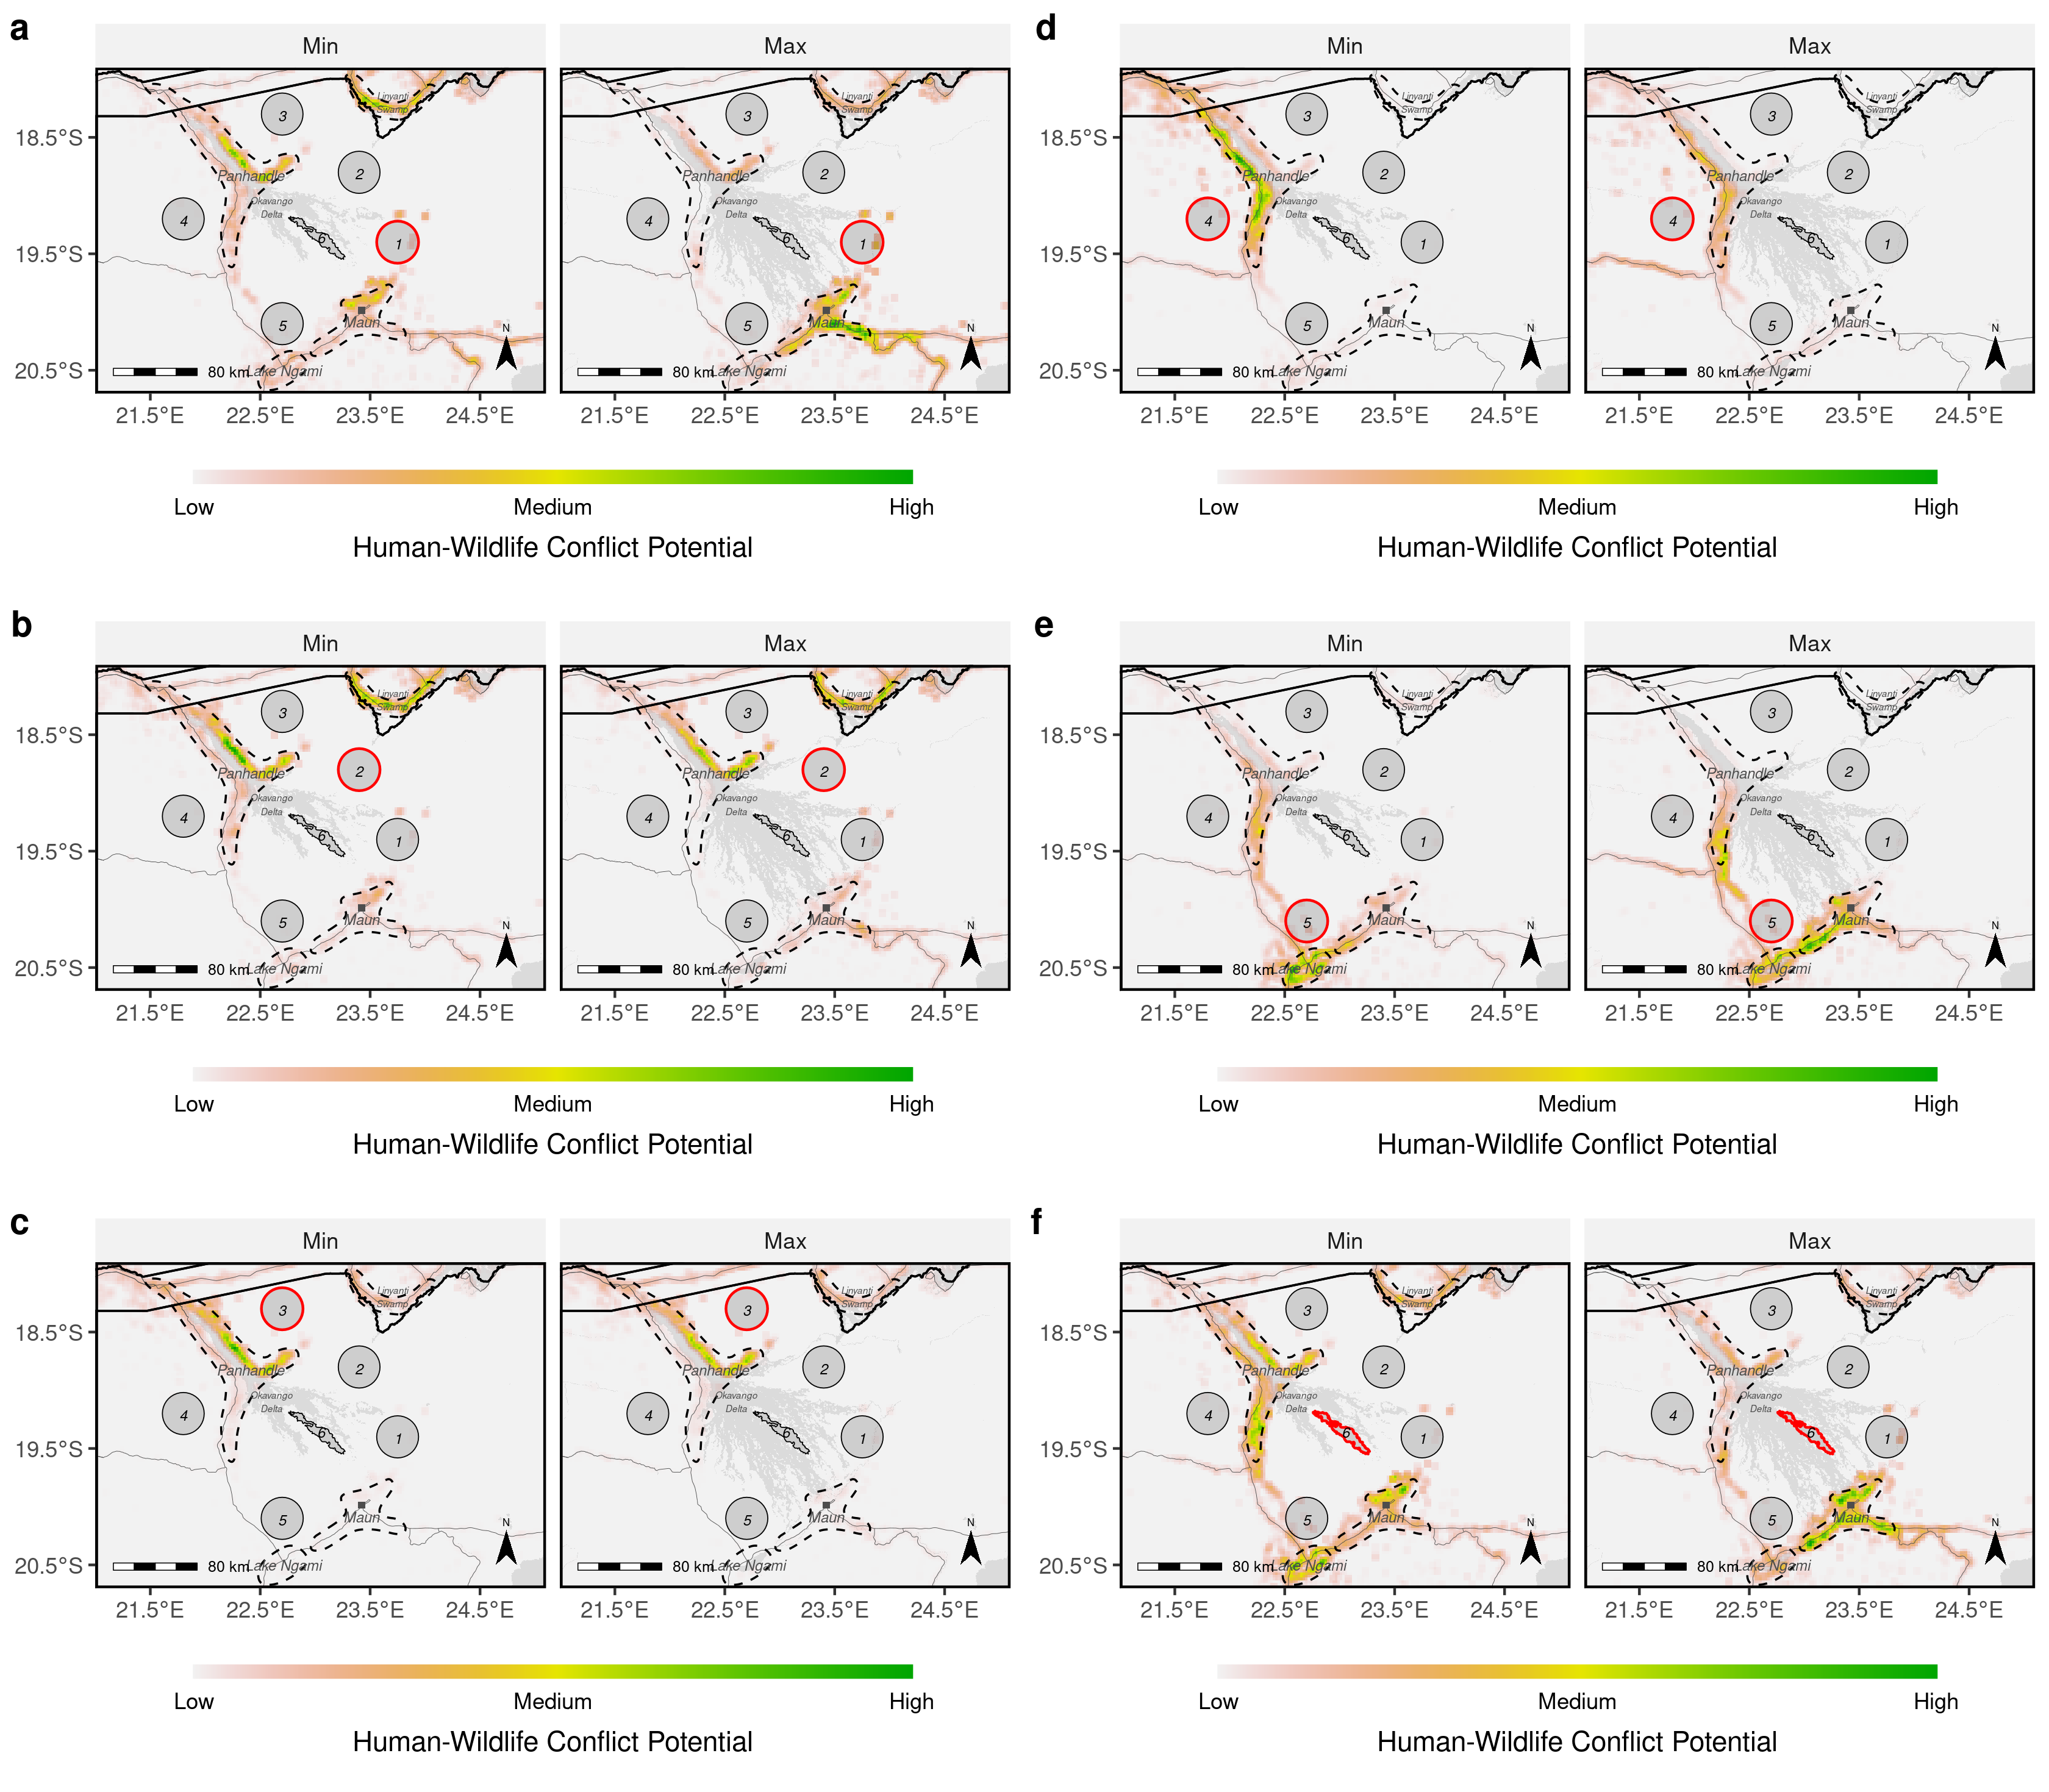
\includegraphics[width = \textwidth]{Figures/HumanWildlifeConflictIndividual.png}
  \caption{Human wildlife conflict maps prepared for each source area separately
  across the two extreme flood-scenarios. The focal source area of each
  subfigure is highlighted by a red circle. Subfigure (a), for instance, depicts
  the human wildlife-conflict maps for source area 1. Dotted shapes were used to
  compare human-wildlife conflict within specific areas (see also Figure S9).}
  \label{HWC}
  \end{center}
\end{figure}

\newpage
\section{Changes in Potential for Human-Wildlife Interactions}
\begin{figure}[htbp]
  \begin{center}
  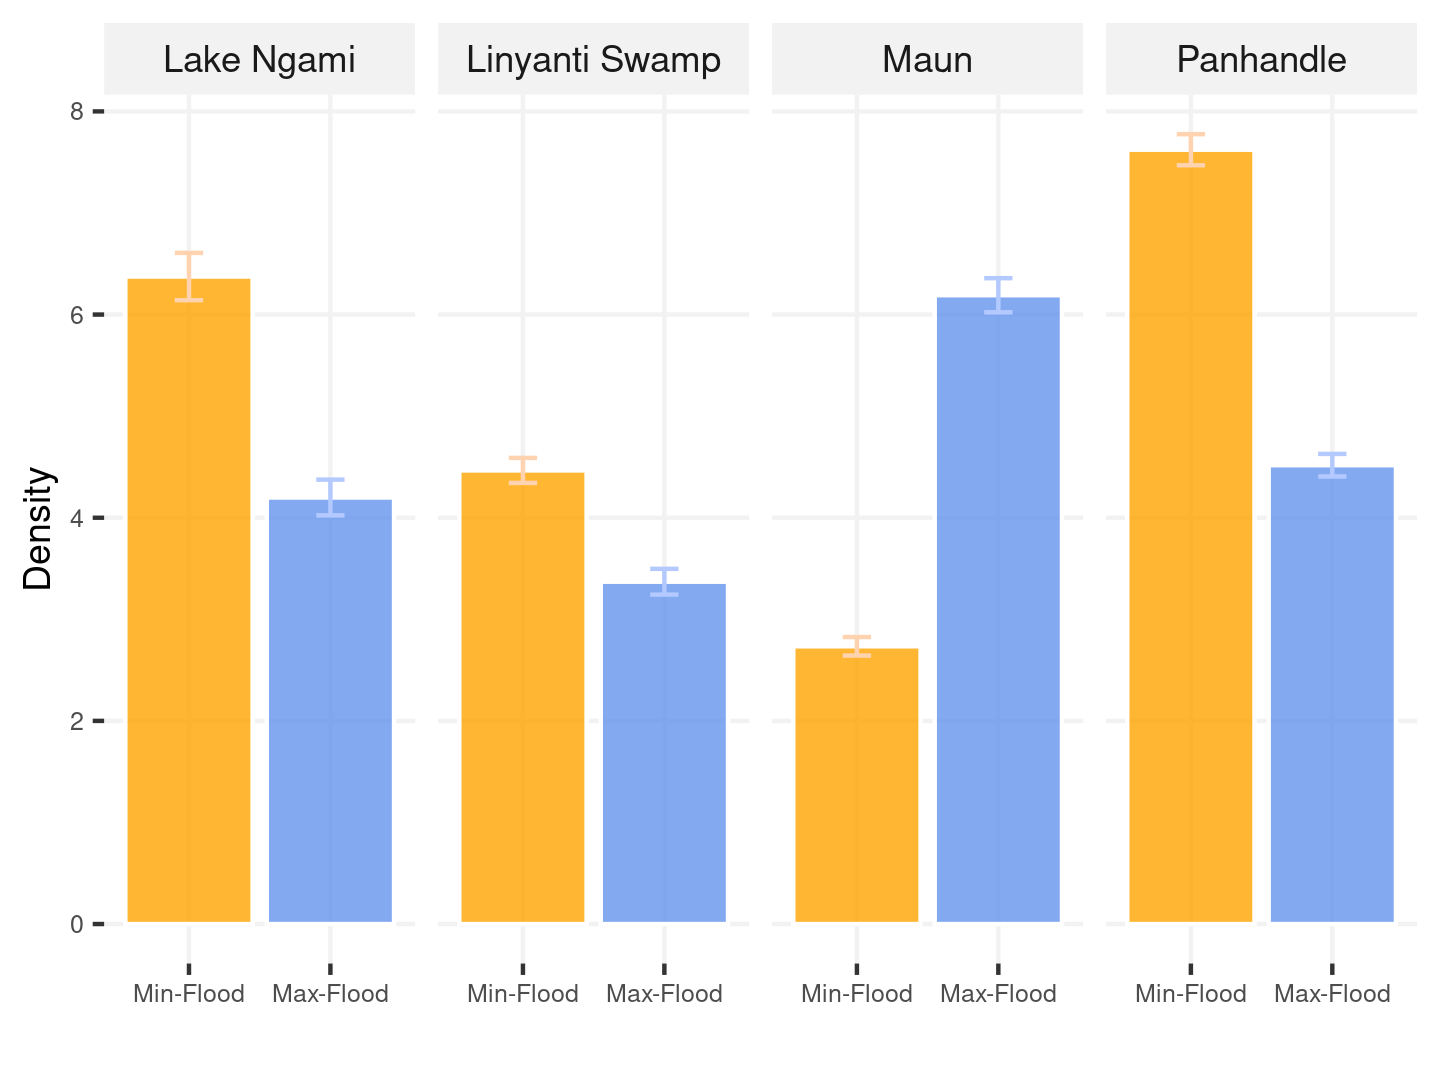
\includegraphics[width = \textwidth]{Figures/HWCDifferenceAOI.png}
  \caption{Number of simulated trajectories within the vicinity of
  human-dominated landcapes in different areas of interest across the minimum
  and maximum flood scenarios. The areas are represented by the black dotted
  shapes in Figure S8}
  \label{HWCDifference}
  \end{center}
\end{figure}

\newpage
\section{Alternative Approach to Map Potential Human-Wildlife Interactions}

To identify potential hotspots for human-wildlife conflict and generate Figure
6c, we isolated all simulated animal locations within 500 meters to a
human-influenced grid-cell (Figure 6c in the main manuscript). To compute the
needed distances, we assumed human-influence to be binary (influence = 1, no
influence = 0), thus ignoring potential impacts of human density. We argue that
the severity of human-wildlife conflict is not necessarily related to human
density, yet humans' attitude towards wildlife. Attitude often correlates
negatively with habitat suitability for the species of interest
\citep{Behr.2017}, and so conflict is often pronounced in peripheral areas
\citep{McNutt.2017}. Since we lacked detailed information of anthropogenic
resistance \citep{Ghoddousi.2021} across the study area, we deemed a binary
representation of human impacts as appropriate. Alternatively, one can also
compute a compound score by multiplying the human-influence layer with the
heatmaps derived from simulated dispersal. This is presented in
\Cref{HWCAlternative}, where we multiplied the heatmaps (\Cref{HWCAlternative}a)
with the human-influence layer (\Cref{HWCAlternative}b) and produced maps
showing potential for human-wildlife conflict. Qualitatively, the maps in
\Cref{HWCAlternative} are very similar to the ones presented in Figure 6c.

\begin{figure}[htbp]
  \begin{center}
  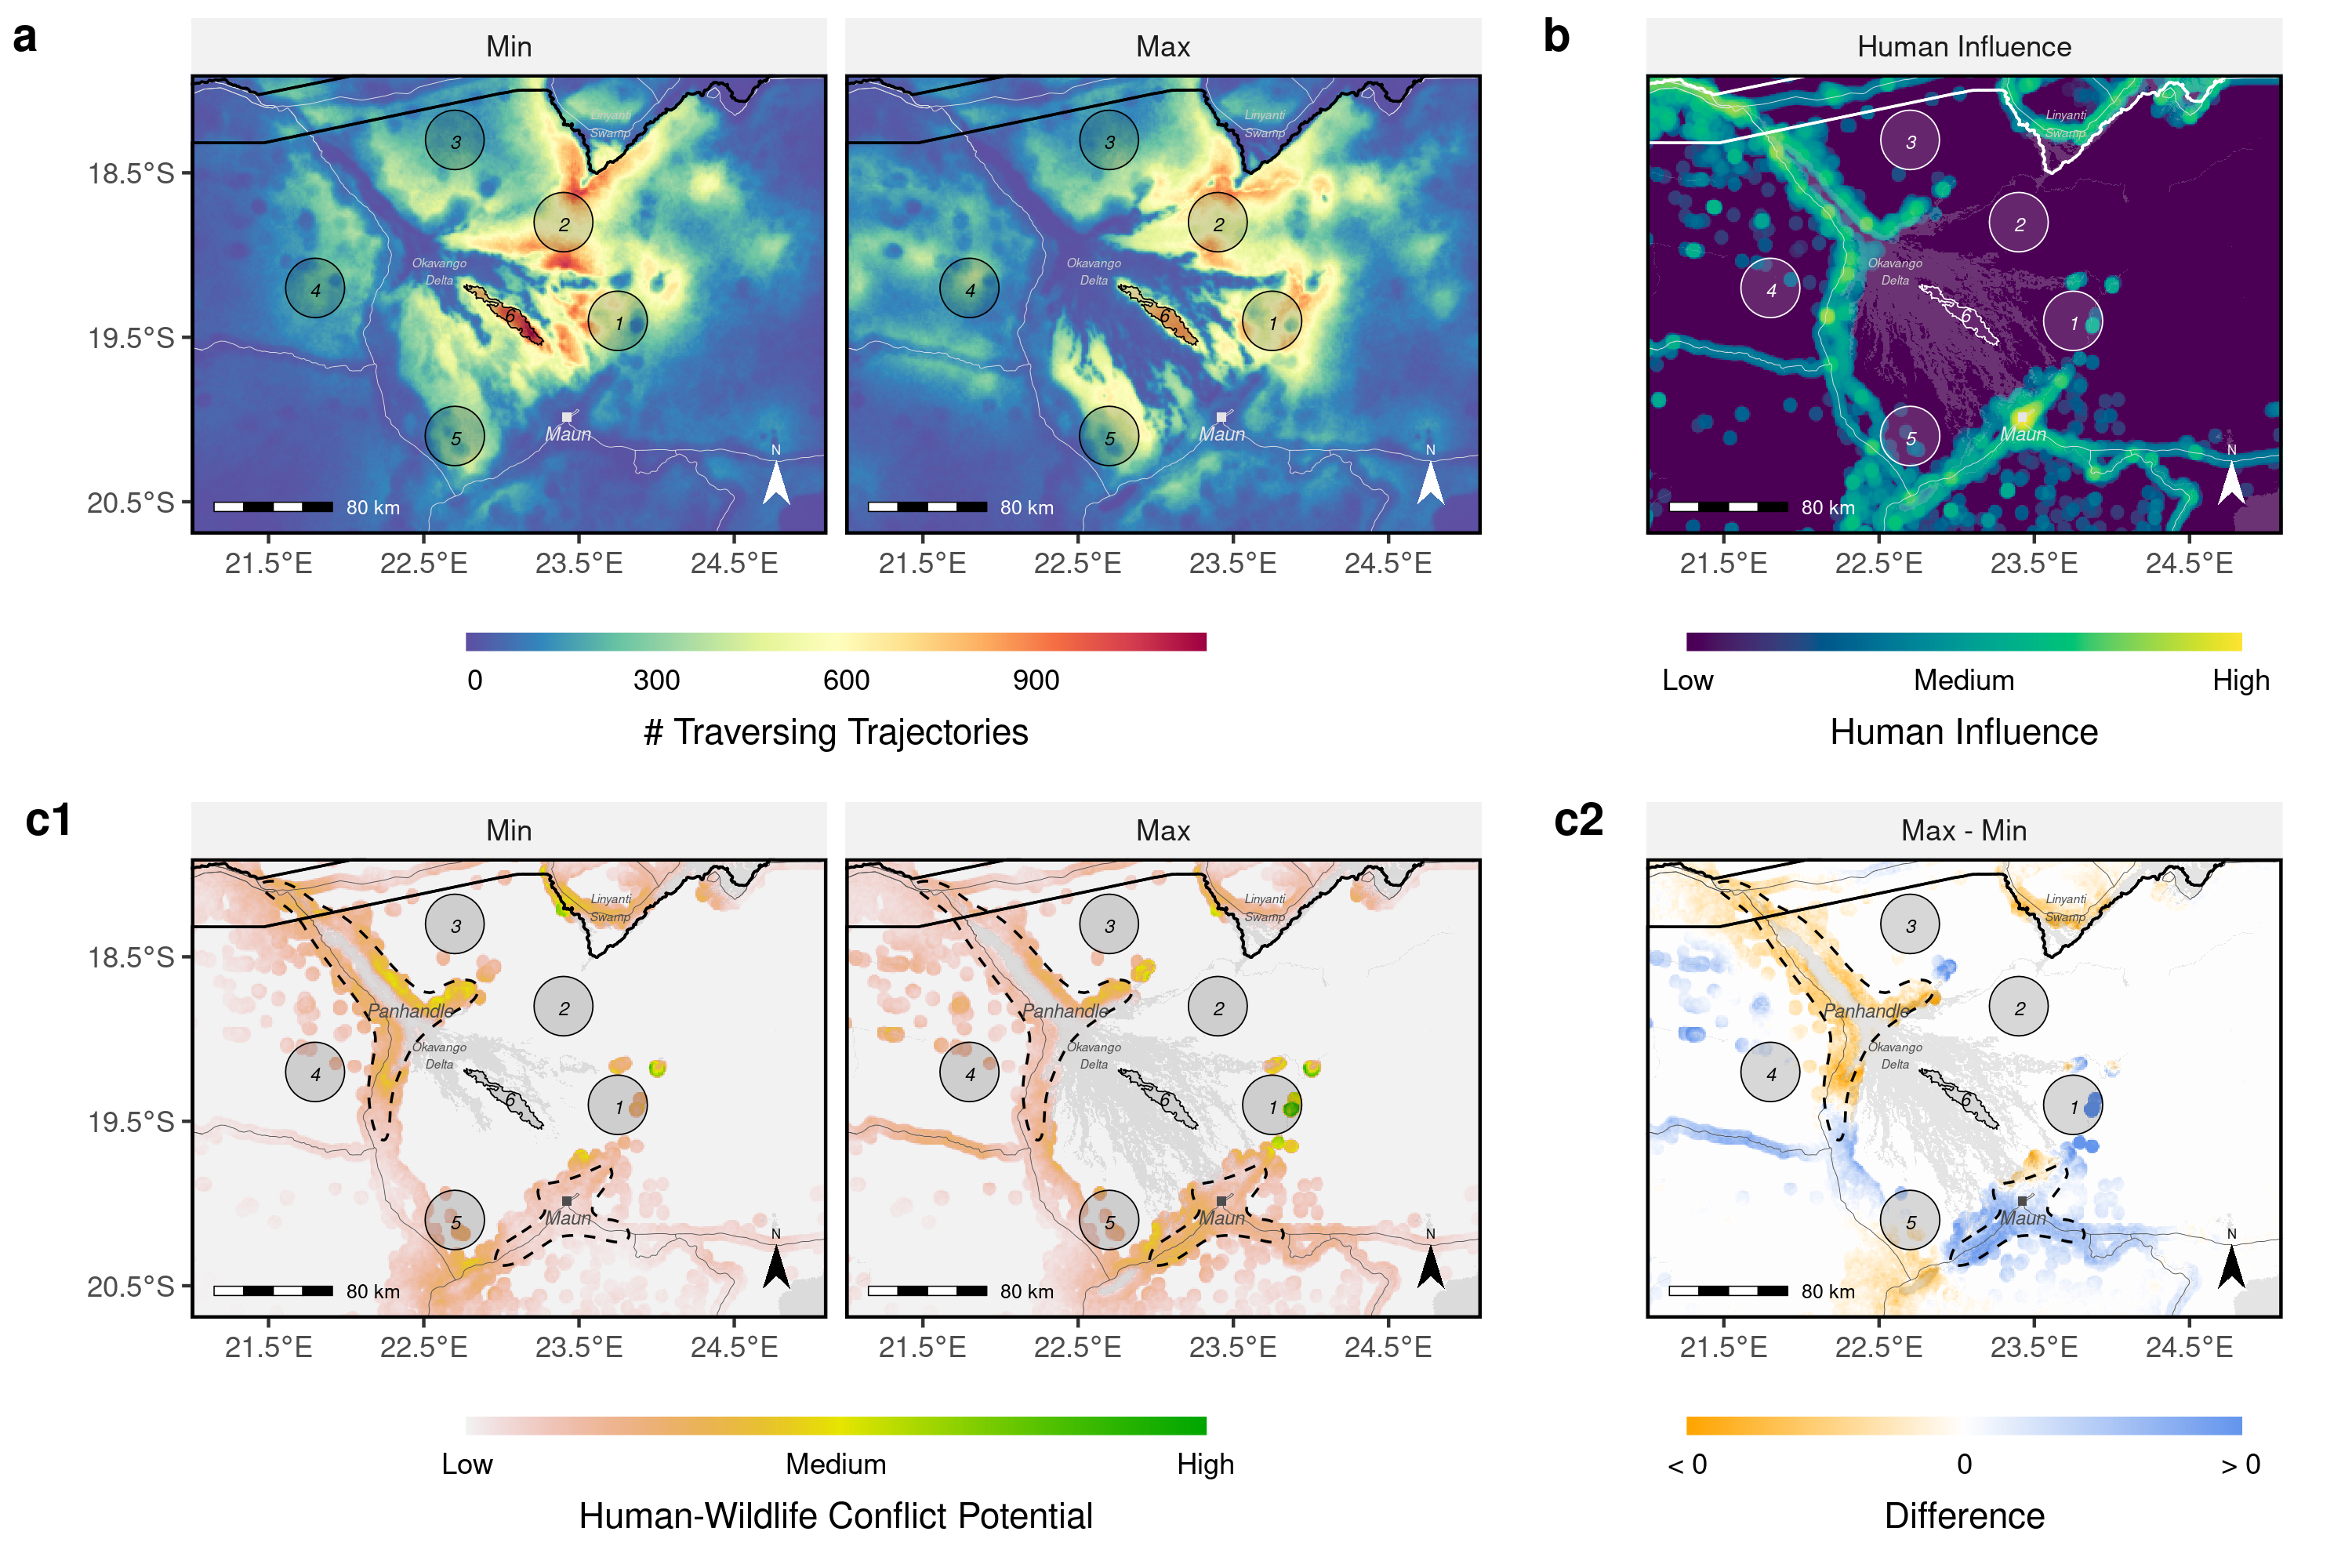
\includegraphics[width = \textwidth]{Figures/HumanWildlifeConflictAlternative.png}
  \caption{Alternative approach to quantifying the potential for human-wildlife
  conflict. Here, we multiplied the heatmaps (a) with the human-influence layers
  (b) to obtain human-wildlife conflict maps (c1). We also computed a difference
  map (c2) for the layers shown in (c1).}
  \label{HWCAlternative}
  \end{center}
\end{figure}

\newpage
\begingroup
\singlespacing
\ifthenelse{\boolean{usebiblatex}}{
  \begin{refcontext}[sorting=nyt]
  \printbibliography
  \end{refcontext}
}{
  \bibliography{LiteratureBibtex}
}
\endgroup
\end{document}
